\chapter[Tau leptons][Tau leptons]{Tau leptons}
\label{chap:taus}

\begin{quote}
  Tau leptons and their signature in the ATLAS detector are described. This draws from extensive ATLAS documentation on the topic~\cite{ATLAS-CONF-2012-142,ATLAS-CONF-2013-064,ATLAS-CONF-2013-044}, especially the recent publication summarizing the Run-I performance~\cite{PERF-2013-06}. These are the featured particles of this thesis.
\end{quote}

% ----------------------------------------------------------------------------------

\section{Tau leptons}
\label{sec:taus-theory}

Tau leptons were discovered in the 1970s by Martin Perl and the SLAC-LBL group at the SPEAR electron-positron collider~\cite{1975.Perl.discovery_of_tau_1,1976.Perl.discovery_of_tau_2,1977.Perl.discovery_of_tau_3}. They have since been studied in great detail at experiments like Belle~\cite{2014.belle.tau-lifetime} and BaBar~\cite{2009.babar.tau-mass}. The associated tau neutrino was first observed directly at the DONUT experiment in 2000~\cite{2001.Kodama.discovery_of_tau_neutrino}, though its existence was inferred by measurements of the width of the $Z$ boson by experiments at the LEP collider in 1990~\cite{1990.ALEPH.3-neutrino-families}.

Tau leptons are the heaviest of the charged leptons. Their mass of 1.78 GeV is approximately twenty times larger than the muon mass~\cite{2012.PDG}, and their short lifetime $c\tau = \text{87 } \micron$ implies tau leptons produced in $pp$ collisions at the LHC typically decay within the ATLAS beam pipe. The ATLAS detector therefore observes only the decay products of the tau lepton, not the particle itself.

Tau leptons decay leptonically ($\tauldecay$) in 35\% of decays and hadronically ($\tauhdecay$) in 65\%. Among hadronic decays, 72\% involve exactly one charged pion and 22\% exactly three charged pions. The remaining percentage of hadronic decays dominantly involves kaons or five (or more) charged pions. All tau lepton decays involve at least one neutrino. A pie chart of tau lepton branching fraction is given in \cref{fig:taus-decaypie}.

\begin{figure}[tp]
  \centering
  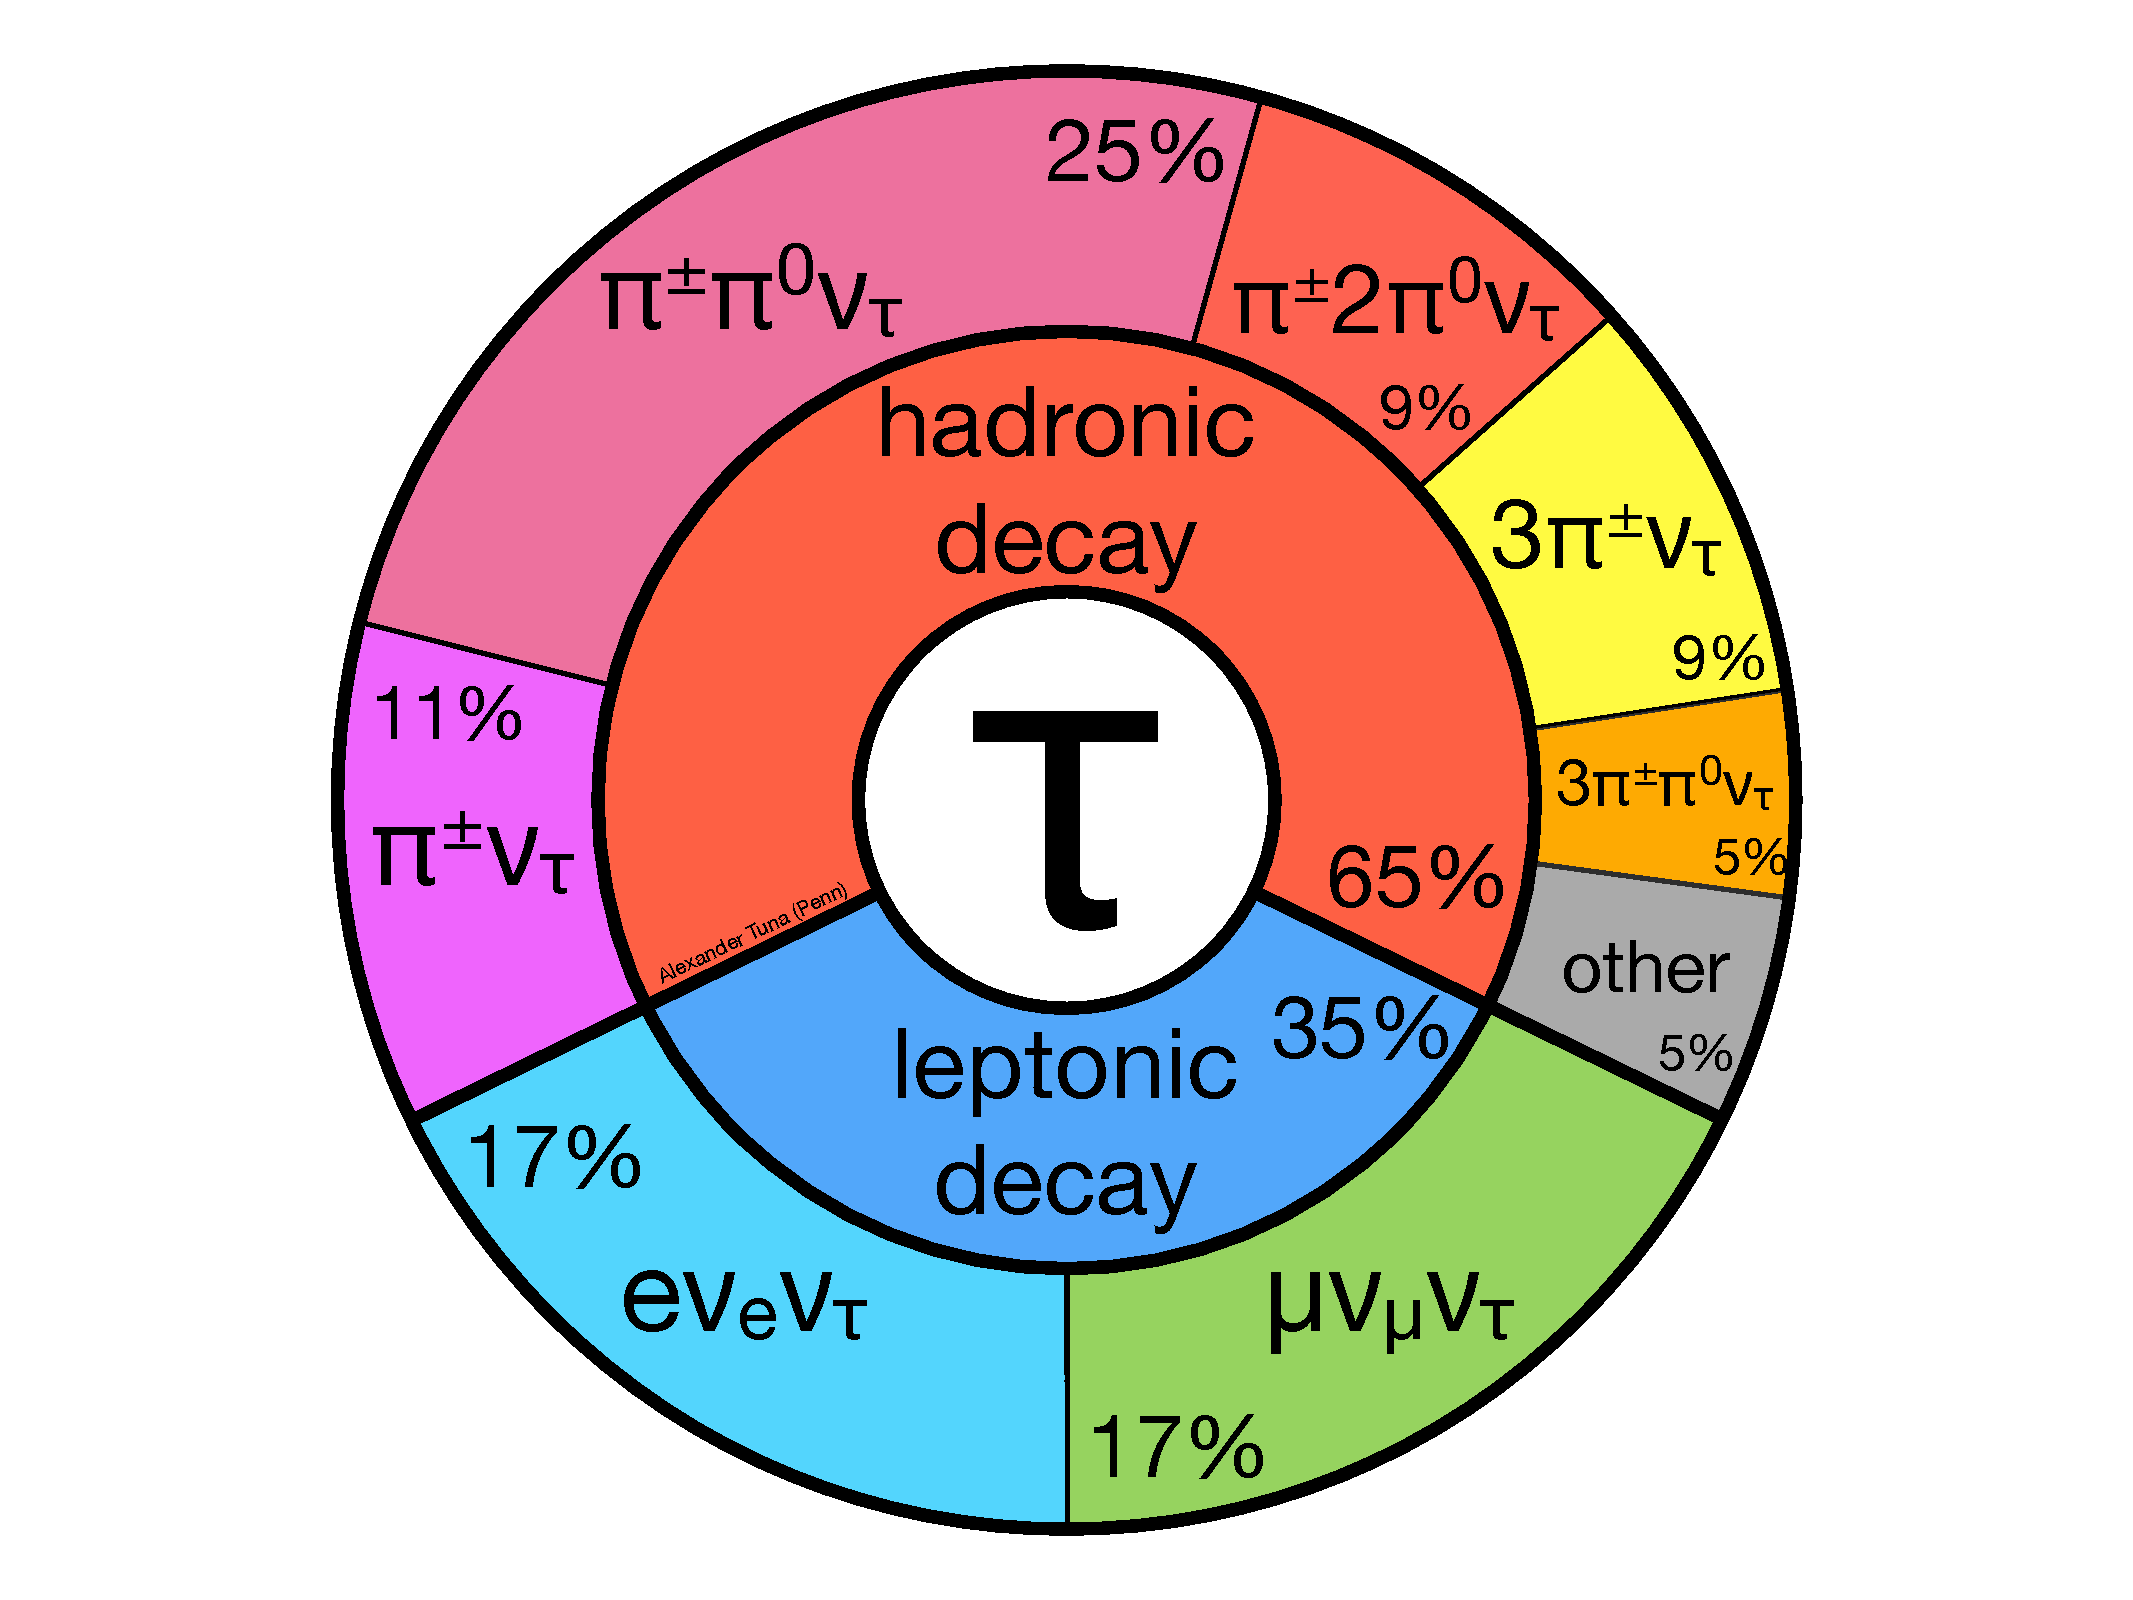
\includegraphics[width=0.48\textwidth]{figures/piecharts/taudecay}
  \caption{Pie chart of tau lepton decay branching fractions, grouped by hadronic decays (65\%) and leptonic decays (35\%).}
  \label{fig:taus-decaypie}
\end{figure}

% ----------------------------------------------------------------------------------

\section{Leptonic tau decays, $\taul$}
\label{sec:taus-leptons}

At ATLAS, light leptons from tau lepton decays ($\tauldecay$) are largely indistinguishable from prompt leptons from $W$ and $Z$ decays. They are typically less energetic due to the presence of two additional neutrinos in the tau lepton decay (e.g., $\Wlv$ versus $\Wtauvlvvv$), but for identification purposes, the only distinguishing features arise from the displaced tau vertex. This displacement is often quantified by the transverse distance of closest approach of the light lepton to the primary vertex ($d_0$). But given the short lifetime of tau leptons, the discrimination power is weak. These properties are shown in \cref{fig:taus-leptonpt}.

\begin{figure}[tp]
  \centering
  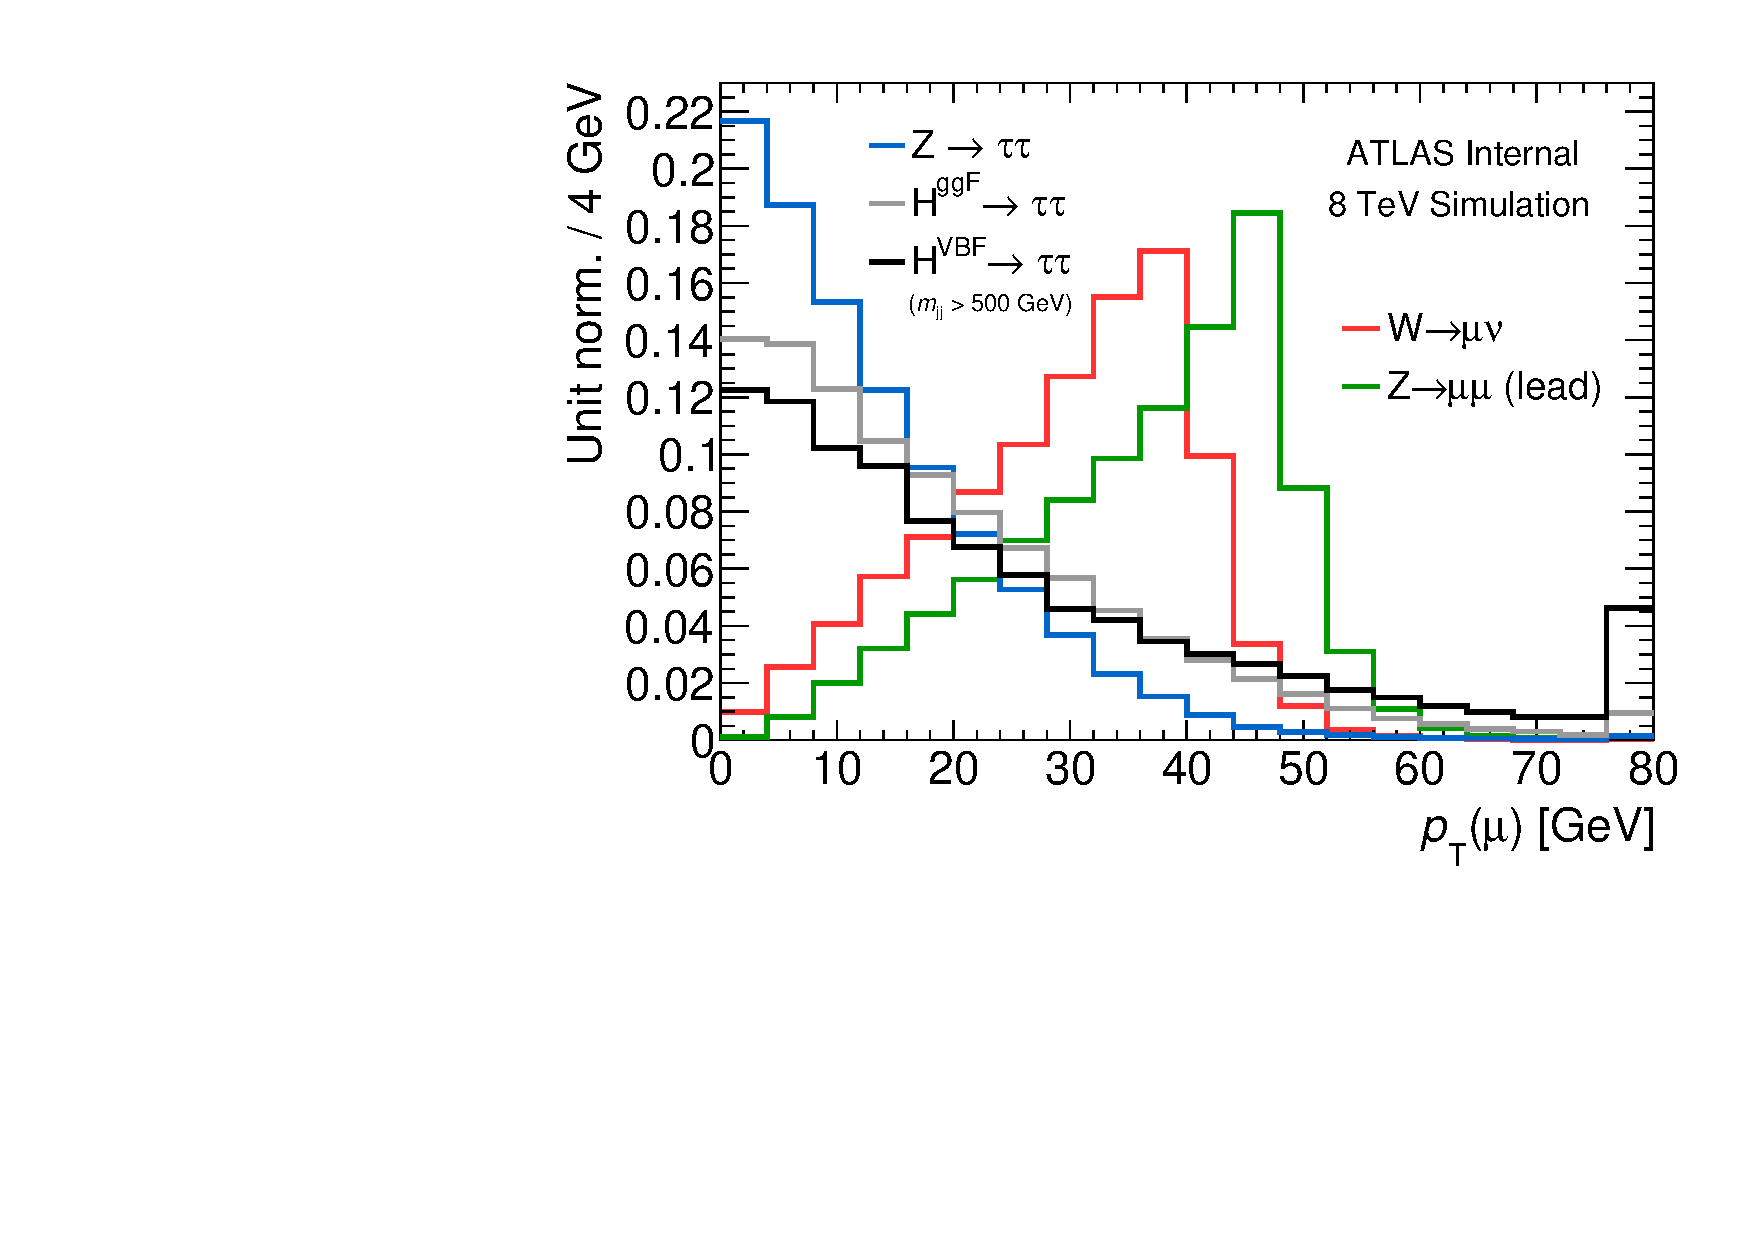
\includegraphics[width=0.48\textwidth]{figures/tauperformance/leptonsfromtausaresoft}
  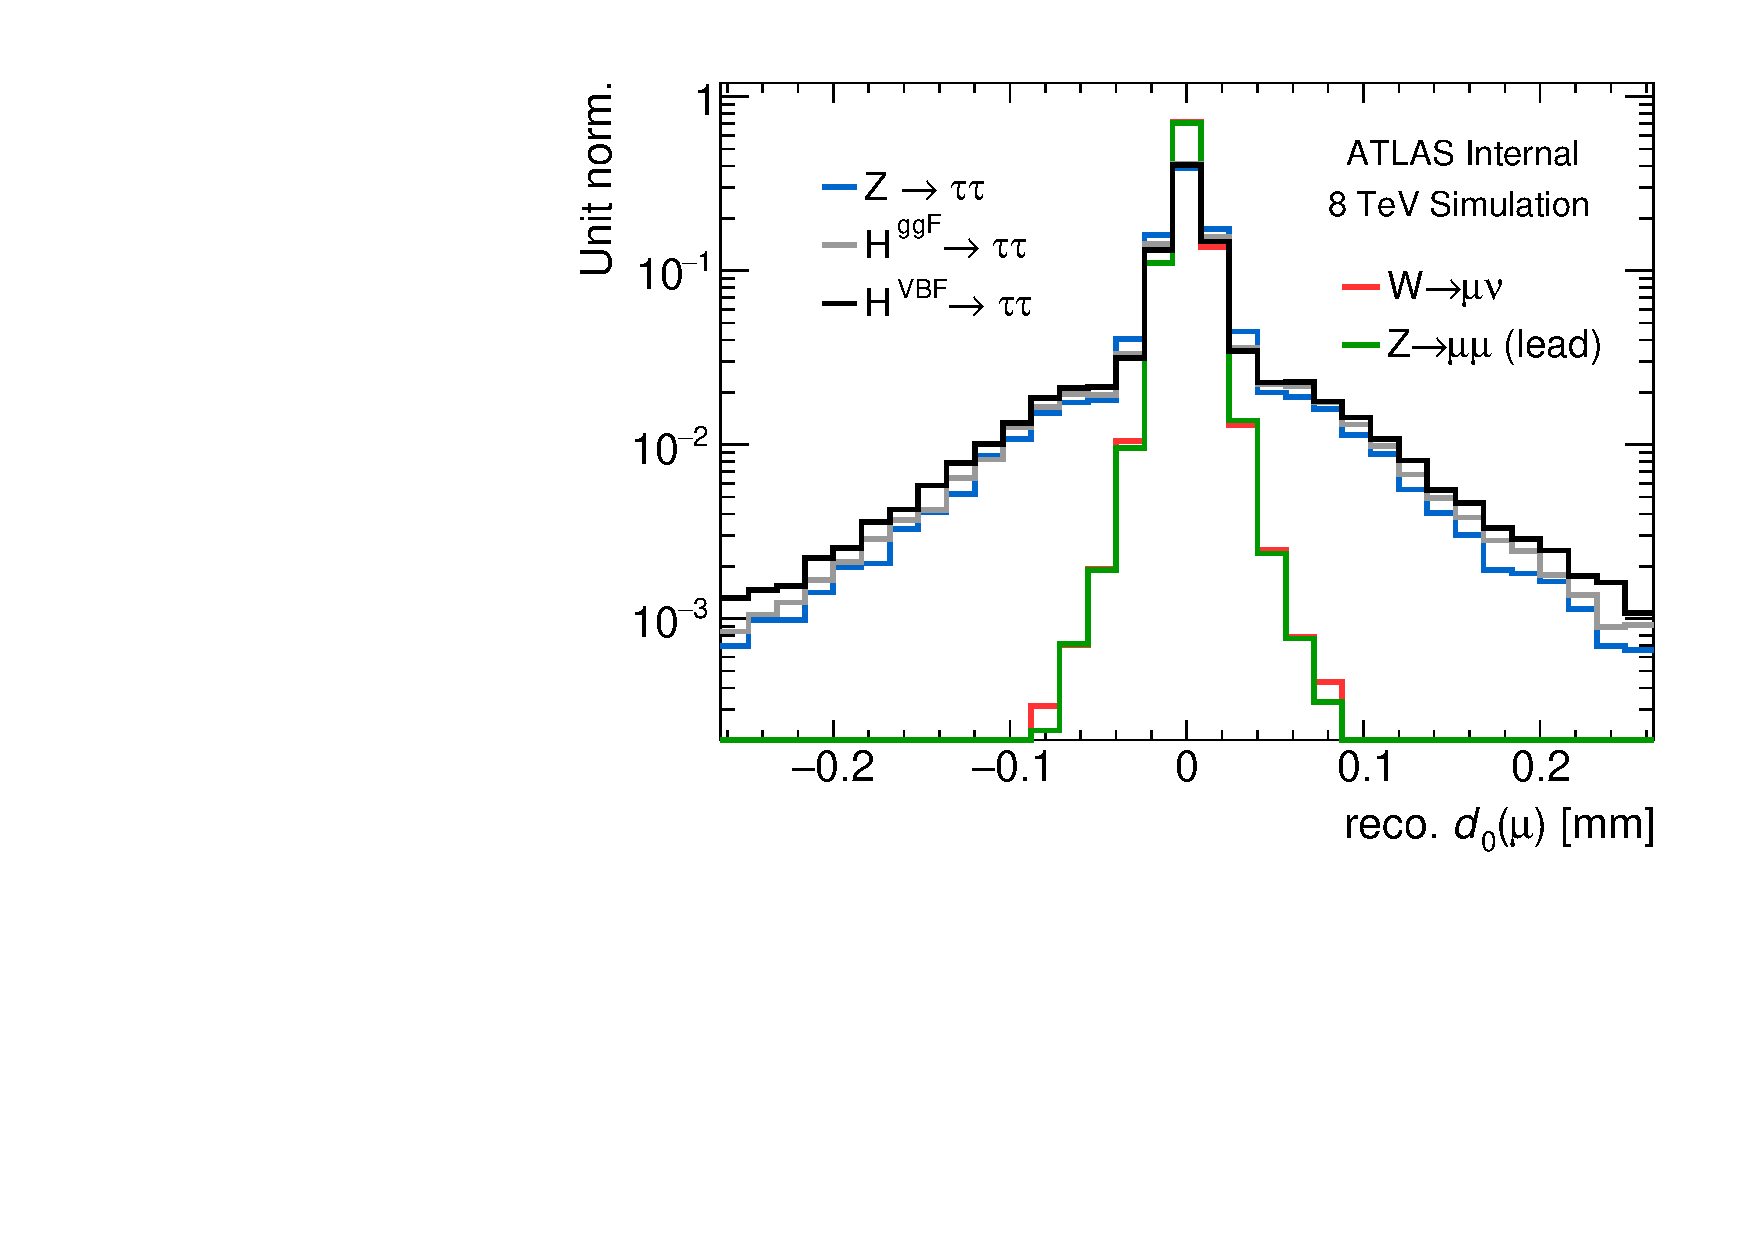
\includegraphics[width=0.48\textwidth]{figures/tauperformance/leptond0}
  \caption{True $\pt$ and reconstructed $d_0$ for muons from simulated $W$, $Z$, and tau lepton decays. Muons from tau lepton decays are shown for $\Ztautau$, $\ggFHtautau$, and $\VBFHtautau$ processes.}
  \label{fig:taus-leptonpt}
\end{figure}

% ----------------------------------------------------------------------------------

\section{Hadronic tau decays, $\tauh$}
\label{sec:taus-hadrons}

This sections follows a recent ATLAS publication describing $\tauh$ performance in Run-I~\cite{PERF-2013-06}.

\subsection{Reconstruction}

% \subsubsection{Calorimeter seeding}

$\tauh$ candidates are seeded by the collection of jets formed by the anti-$k_t$ algorithm with distance parameter $R=0.4$, which groups the set of reconstructed three-dimensional calorimeter TopoClusters into jet objects. These TopoClusters are calibrated using a local hadronic calibration (LC). Jets are required to have $\pt > 10 \GeV$ and $|\eta| < 2.5$ to qualify as a seed for a $\tauh$ candidate. The initial $\tauh$ four-momentum is calculated by summing the TopoClusters within $\Delta R < 0.2$ of the barycenter of the jet seed, where the $\tauh$ mass is assume to be zero.

% \subsubsection{Track and vertex association}

Tracking and vertexing for $\tauh$ occurs in three steps. First, all tracks are collected within $\Delta R < 0.2$ of the jet seed which pass quality criteria described later, but for which no impact parameter requirements are made. Second, the tau vertex (TV) is defined as the reconstructed vertex which maximizes the fraction of track momenta originating from that vertex versus total track momenta, referred to as the tau vertex fraction:
%
\begin{equation}
  \begin{split}
    \text{TVF}(\text{vertex}) &= \frac{\sum \pt^\text{tracks associated to vertex}}{\sum \pt^\text{tracks}} \\
  \end{split}
  \label{eqn:taus-tvf}
\end{equation}
%
This vertex association is called the Tau Jet Vertex Association (TJVA) algorithm, and it helps ensure robustness against harsh pileup conditions, as shown in \cref{fig:taus-tjva}.

\begin{figure}[tp]
  \centering
  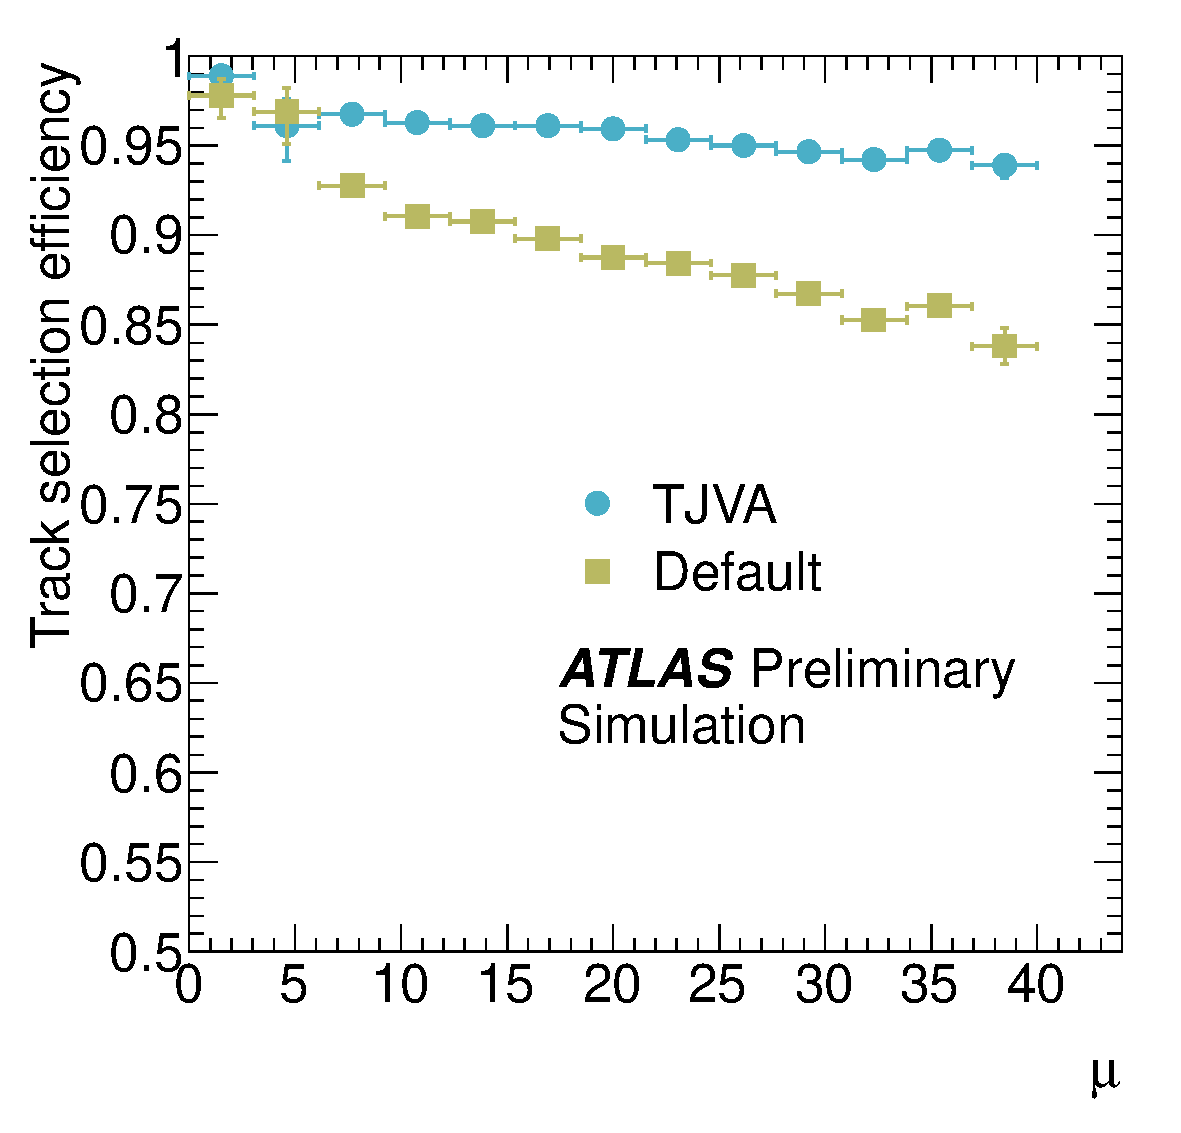
\includegraphics[width=0.48\textwidth]{figures/ATLAS-CONF-2012-142/fig_01a}
  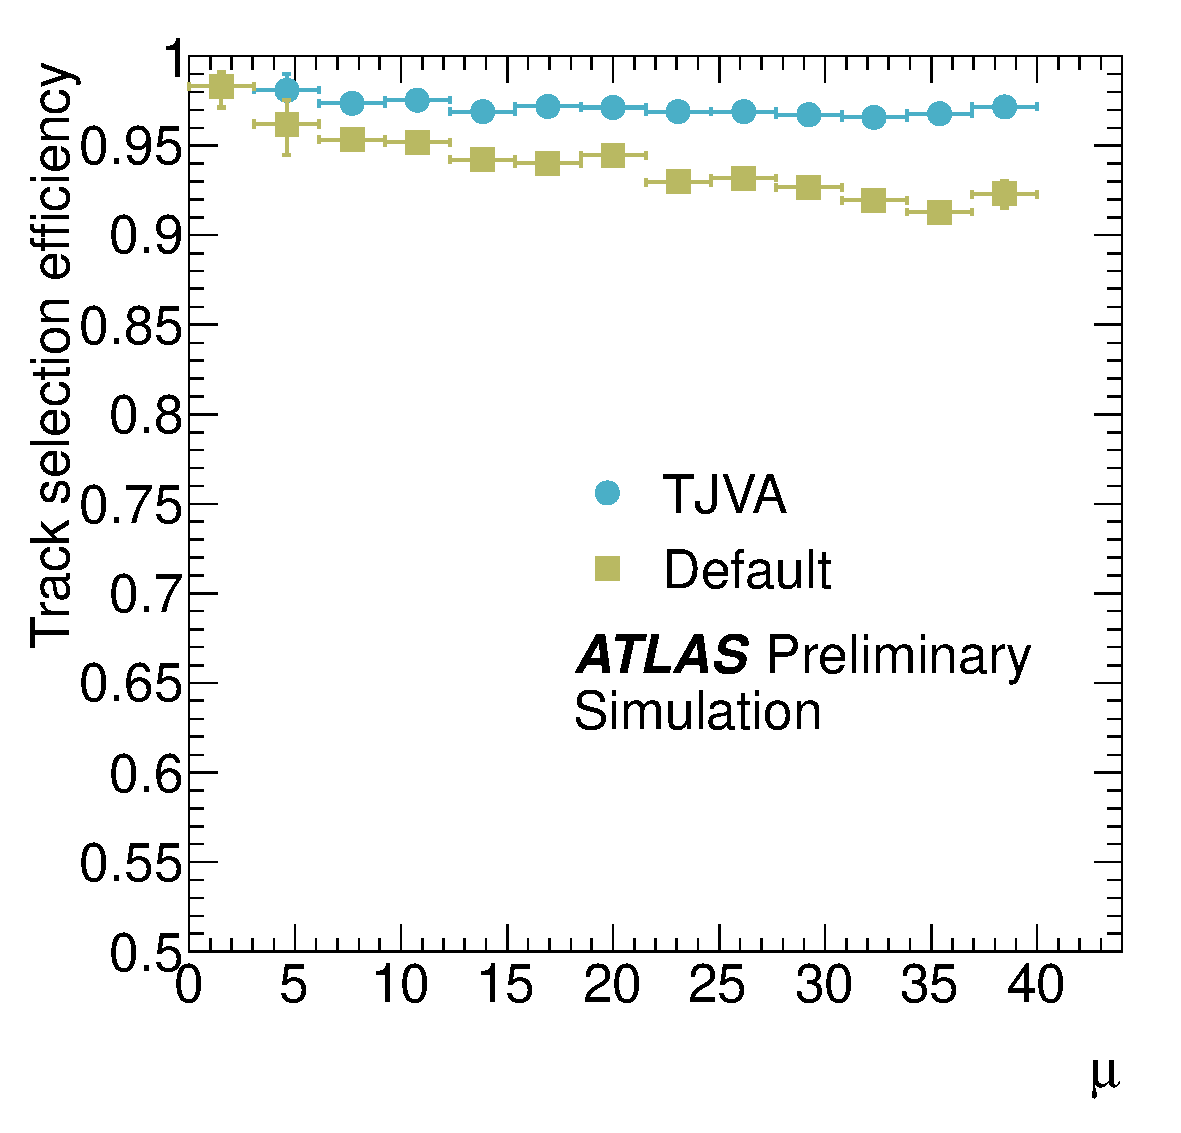
\includegraphics[width=0.48\textwidth]{figures/ATLAS-CONF-2012-142/fig_01b}
  \caption{Track selection efficiency for $\tauh$ candidates with the default vertex selection (highest $\Sigma\pt^2$) versus the dedicated TJVA algorithm, for true 1-track (left) and 3-track (right) $\tauh$, as a function of $\pileup$~\cite{ATLAS-CONF-2012-142}.}
  \label{fig:taus-tjva}
\end{figure}

Last, the set of tracks is reduced by making additional impact parameters requirements with respect to the TV. The full set of track selection criteria are:
%
\begin{itemize}
    \item $\pt > 1~\mathrm{GeV}$,
    \item at least two hits in the pixel subdetector,
    \item at least seven hits in the pixel and SCT subdetectors combined,
    \item $|d_{0,\text{TV}}| < 1.0~\mathrm{mm}$,
    \item $|z_{0,\text{TV}} \, \sin{\theta}| < 1.5~\mathrm{mm}$
\end{itemize}
%
This set of tracks is used when classifying the $\tauh$ candidate track multiplicity. For identification purposes, tracks in the \textit{isolation region} $0.2 < \Delta R < 0.4$ are also required to pass these criteria.

% \subsubsection{Calibration}

A correction to the $\tauh$ energy is applied to account for biases, such as effects from pileup, the underlying event, and clusters falling out of the $\Delta R = 0.2$ cone. This correction is derived in simulated $\Ztautau$, $\Wtaunu$, and $\Zptautau$ events where the true visible $\tauh$ energy $\Etruevis$ is known. It is derived as a function of the pre-calibrated $\tauh$ energy $\ErecoLC$ and $\eta$ and shown in \cref{fig:taus-calibration}. Small additional corrections are applied to account for biases from pileup and poorly instrumented regions of the detector. The resulting $\tauh$ energy resolution is shown in \cref{fig:taus-resolution}.

\begin{figure}[tp]
  \centering
  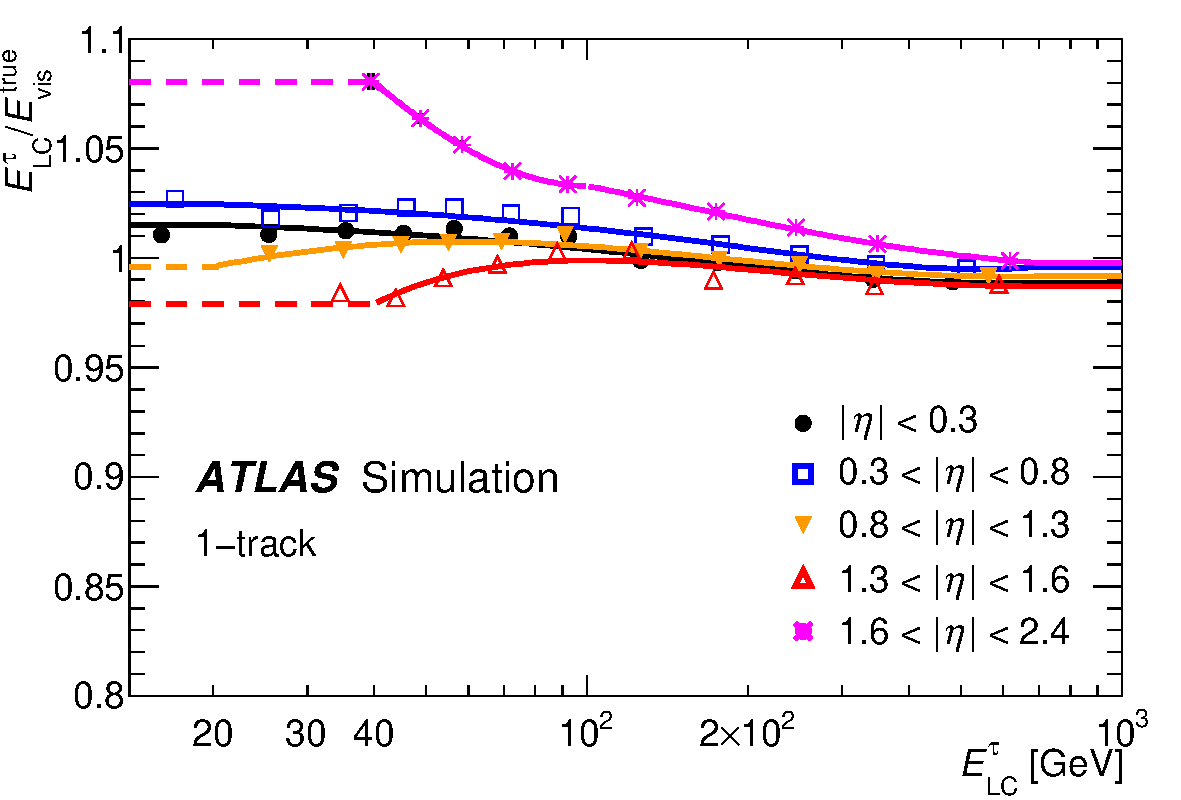
\includegraphics[width=0.48\textwidth]{figures/PERF-2013-06/fig_15a}
  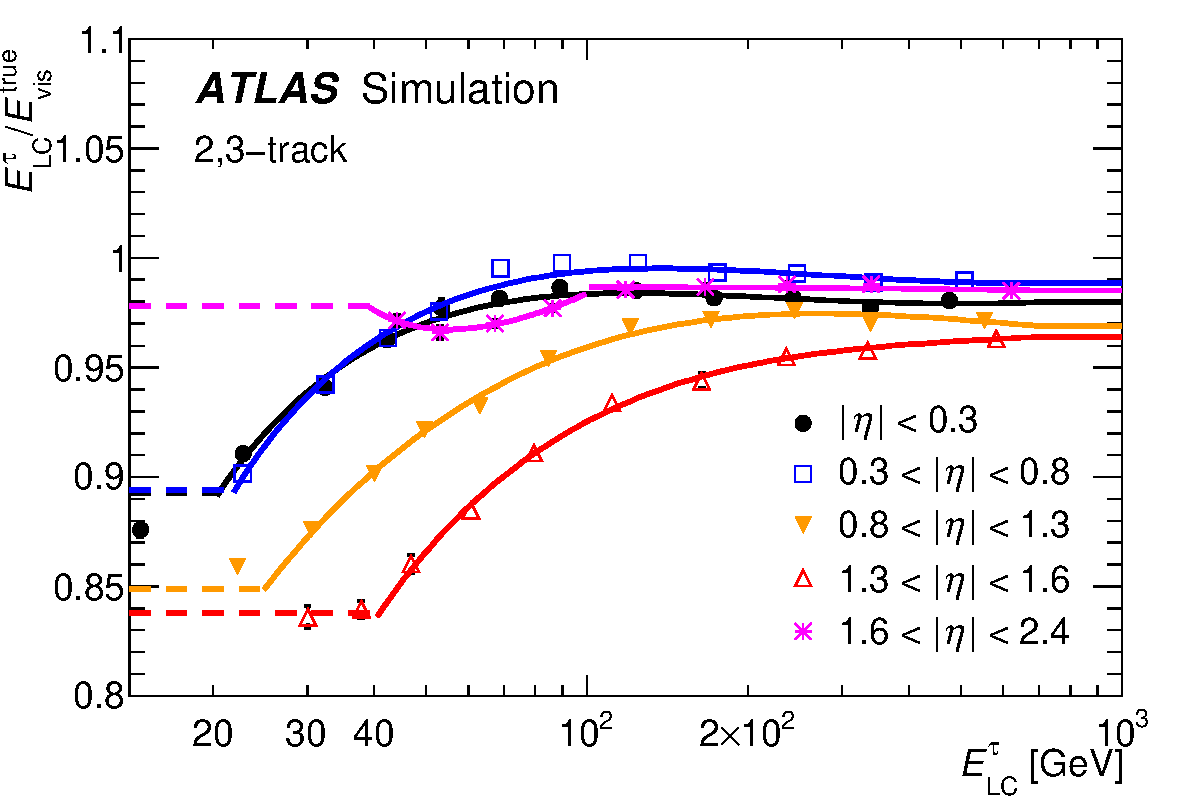
\includegraphics[width=0.48\textwidth]{figures/PERF-2013-06/fig_15b}
  \caption{$\tauh$ energy response curves measured in simulation, for 1-track (left) and 2,3-track (right) $\tauh$, as a function of the reconstructed energy~\cite{PERF-2013-06}.}
  \label{fig:taus-calibration}
\end{figure}

\begin{figure}[tp]
  \centering
  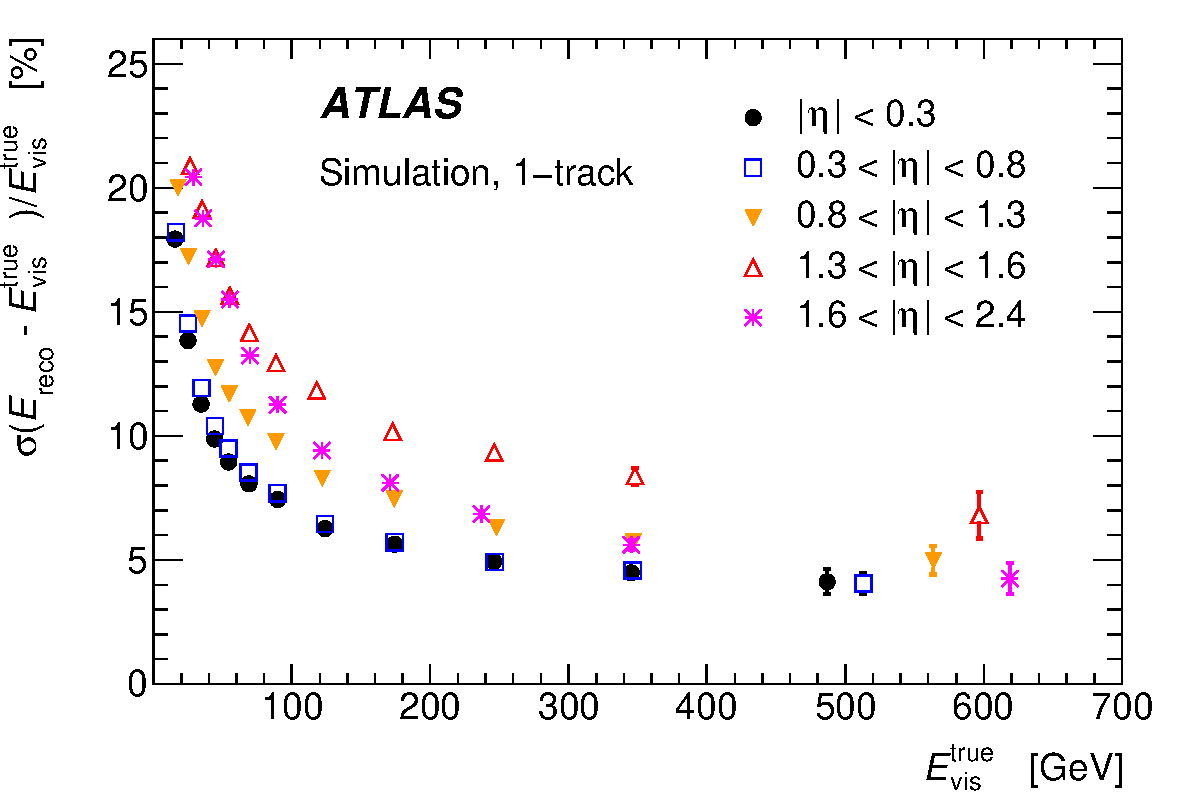
\includegraphics[width=0.48\textwidth]{figures/PERF-2013-06/fig_16a}
  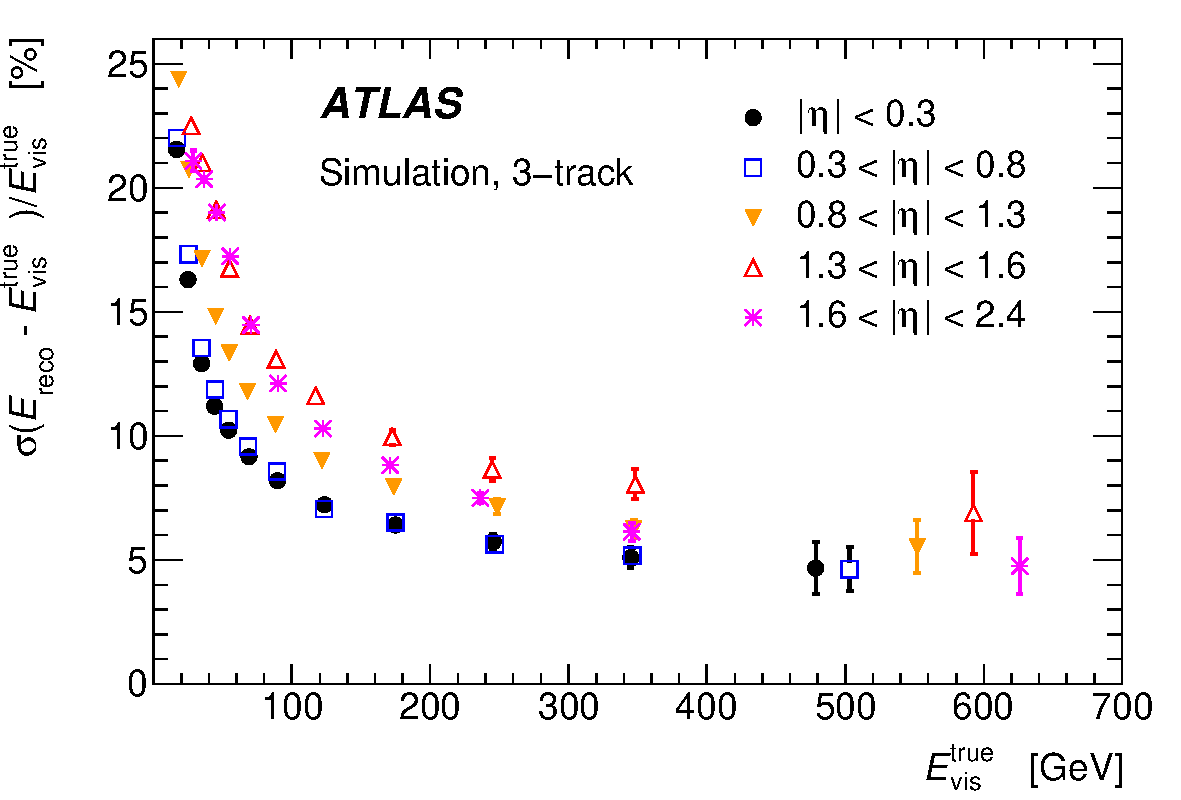
\includegraphics[width=0.48\textwidth]{figures/PERF-2013-06/fig_16b}
  \caption{$\tauh$ energy resolution measured, for 1-track (left) and 2,3-track (right) $\tauh$, as a function of the true visible energy~\cite{PERF-2013-06}.}
  \label{fig:taus-resolution}
\end{figure}

Data-driven corrections for and uncertainties on the $\tauh$ energy calibration are derived in two ways: the \textit{deconvolution method} and the \textit{in-situ} method. The deconvolution method relies on the $\tauh$ having a known composition of charged and neutral hadrons such that the response can be decomposed into individual sources. For charged hadrons, the response is estimated from test beam measurements and simulation with varied hadronic shower models. For electromagnetic showers from neutral pion decays, the response is estimated from $\Zee$.

The in-situ method relies on the sensitivity of the visible $\mtautau$ in $\Ztaultauh$ events to the $\tauh$ energy. Relative to $\tauh$, the lepton energy is precisely calibrated and validated in data with $\Zll$ events. These events are selected in data by requiring exactly one isolated muon, exactly one identified $\tauh$, and some additional kinematic cuts to suppress non-$\Ztaultauh$ events. The $\tauh$ energy is then allowed to float like $(1 + \alpha)E_\text{T}$, and the effect is propagated to the visible $\mtautau$ spectrum. The data is then adjusted by the parameter $\alpha$ to match the simulated prediction, which has already been corrected to $\Etruevis$. The measured $\alpha$, called the \textit{TES shift}, is:
%
\begin{equation}
  \begin{split}
    \alpha_\text{1-track} &= 0.8\% \pm 1.3\% \text{ (stat.)} \pm 0.6\% \text{ (syst.) } \\
    \alpha_\text{3-track} &= 1.1\% \pm 1.4\% \text{ (stat.)} \pm 0.7\% \text{ (syst.) } \\
  \end{split}
  \label{eqn:taus-tesshift}
\end{equation}
%

\subsection{Identification}

As a high energy hadron collider, the overwhelming majority of particles observed by ATLAS are hadrons. Distinguishing these QCD jets from $\tauh$ is hugely important for physics with tau leptons. The properties with discriminating power can be broadly grouped into three categories:
%
\begin{description}
    \item[Track multiplicity:] \hfill \\
      $\tauh$ tend to have 1 or 3 associated tracks, where no such specificity is expected for jets.
    \item[Narrowness:]         \hfill \\
      $\tauh$ tend to be more narrow in the tracker and calorimeter since tau leptons from electroweak decays are boosted.
    \item[Displaced vertex:]   \hfill \\
      Tracks from $\tauh$ tend to be more displaced from the primary vertex than tracks in jets due to the finite tau lepton lifetime.
\end{description}
%
The track multiplicity and narrowness features are shown in \cref{fig:taus-eventdisplay}.

\begin{figure}[tp]
  \centering
  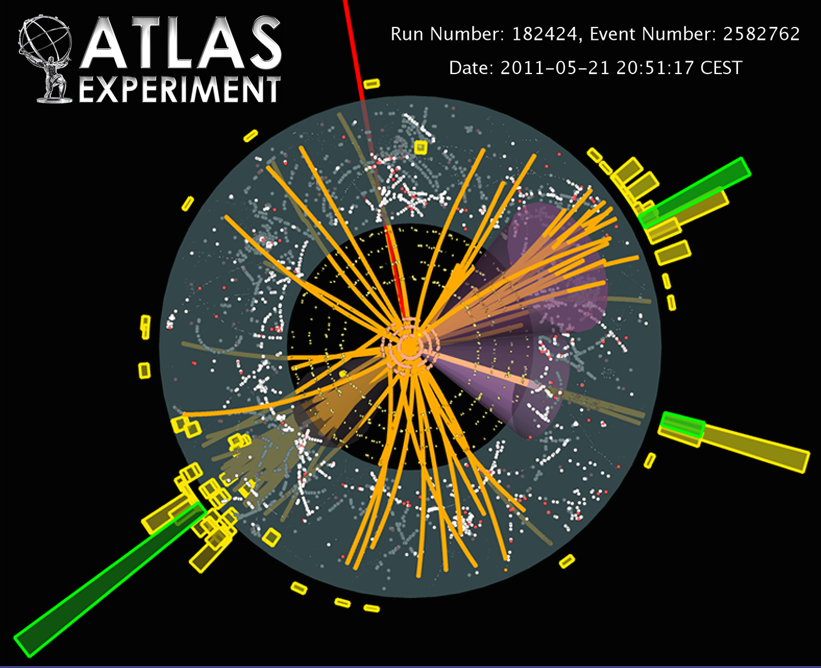
\includegraphics[width=0.95\textwidth]{figures/tauperformance/vp1_3dcocktail_run182424_evt2582762_tttaumu}
  \caption{Event display of a $tt \rightarrow (b\mu\nu_\mu)(b\tauh\nu_\tau)$ candidate during 2011 data-taking~\cite{atlas-eventdisplays}. The $\tauh$ candidate has 3 tracks, the $b$-jet candidates each have more than 10 tracks, and the muon is in red. The estimated purity of the selection is greater than 75\%.}
  \label{fig:taus-eventdisplay}
\end{figure}

For track multiplicity, reconstructed $\tauh$ are required to have exactly 1 or 3 associated tracks. This is effective at rejecting QCD jets which have a broader track multiplicity spectrum. This requirement has signficant efficiency loss (20-40\%) due to photon conversions from neutral pion decays and pileup, among other effects. The track multiplicity spectrum for $\tauh$ and jets is shown in \cref{fig:taus-trackmultiplicity} in a $\Ztaultauh$-rich selection of data.

\begin{figure}[tp]
  \centering
  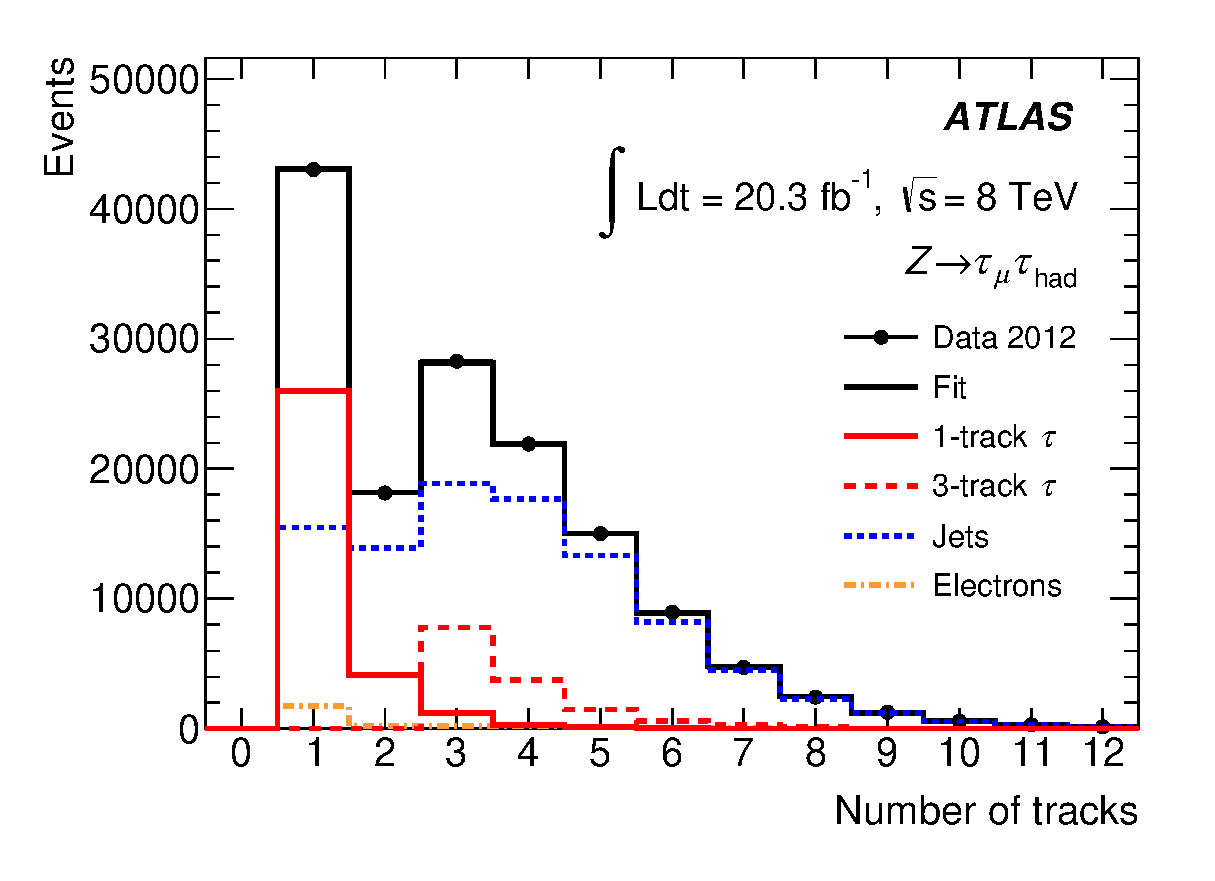
\includegraphics[width=0.95\textwidth]{figures/PERF-2013-06/fig_10a}
  \caption{Fit of the predicted $\tauh$ track multiplicity to data in a $\Ztautaumh$ event selection before applying tau identification algorithms~\cite{PERF-2013-06}. The $\tauh$ candidates have much lower track multiplicity relative to the large jet background.}
  \label{fig:taus-trackmultiplicity}
\end{figure}

For narrowness and vertex displacement, discriminating variables are formed using tracking and calorimeter information and combined in multi-variate identification algorithms. These algorithms are typically referred to as $\tauh$ identification or jet discriminators. A complete description of the variables used is given in \cref{tab:taus-idvars} and \cref{apx:tauid}.

An additional identification algorithm is used to decompose the tau lepton decay into charged and neutral pions. The algorithm is sequential: first, it uses global $\tauh$ features measured in the tracker and calorimeter to reconstruct the number of neutral pions associated to the $\tauh$. Second, it creates neutral pion candidates from the most $\pi^0$-like clusters associated to the $\tauh$. These candidates, along with the charged pions measured as associated tracks, make up the decomposed $\tauh$ and feed into the jet discriminant. This reconstruction is substantially more difficult than for charged pions which enjoy precision measurements in the tracker with marginal contamination from pileup, the underlying event, and other processes.

\begin{description}

    \item[Central energy fraction (\centEnergyFrac{}):] \hfill \\ 
      Fraction of transverse energy deposited in the region $\Delta R < 0.1$ out of all energy deposited in the region $\Delta R < 0.2$ around the $\tauh$ candidate calculated by summing the energy deposited in all cells belonging to TopoClusters with a barycenter in this region, calibrated at the EM energy scale. Biases due to pile-up contributions are removed using a correction based on the number of reconstructed primary vertices in the event.

    \item[Leading track momentum fraction (\leadTrackMomFrac{}):] \hfill \\ 
      The transverse momentum of the highest-\pt{} charged particle in the core region of the $\tauh$ candidate, divided by the transverse energy sum, calibrated at the EM energy scale, deposited in all cells belonging to TopoClusters in the core region. A correction depending on the number of reconstructed primary vertices in the event is applied to this fraction, making the resulting variable pile-up independent.

    \item[Track radius (\trackRadius{}):] \hfill \\ 
      \pt-weighted distance of the associated tracks to the $\tauh$ direction, using all tracks in the core and isolation regions.

    \item[Leading track IP significance (\ipSigLeadTrk{}): ] \hfill \\ 
      Transverse impact parameter of the  highest-\pt{} track in the core region, divided by its estimated uncertainty.

    \item[Number of tracks in the isolation region (\numIsoTrack{}):] \hfill \\ 
      Number of tracks associated to the $\tauh$ in the region $0.2<\Delta R<0.4$.
      
    \item[Maximum $\Delta R$ (\dRmax{}): ] \hfill \\ 
      The maximum $\Delta R$ between a track associated to the $\tauh$ candidate and the $\tauh$ direction. Only tracks in the core region are considered.
      
    \item[Transverse flight path significance (\transFlightSig{}):] \hfill \\ 
      The decay length of the secondary vertex (vertex reconstructed with the tracks associated to the core region of the $\tauh$ candidate) in the transverse plane, divided by its estimated uncertainty. It is defined only for multi-track $\tauh$ candidates.
      
    \item[Track mass (\trackMass{}):] \hfill \\ 
      Invariant mass of the four-vector sum of the charged particle momenta in the core and isolation regions.
      
    \item[Track-plus-$\pi^0$-system mass (\trackPizeroMass{}):] \hfill \\ 
      Invariant mass of the system composed of the tracks and $\pi^0$ mesons in the core region.
      
    \item[Number of $\pi^0$ mesons reconstructed in the core region ($N_{\mathrm{\pi^0} } $).] \hfill 
      
    \item[Ratio of track-plus-$\pi^0$-system \pt{} to total $\tauh$ \pt{} (\Etratio{}): ] \hfill \\ 
      Ratio of estimated \pt{} using track + $\pi^0$ information to the calorimeter-only measurement.
      
\end{description}

\begin{table}[bp] 
  \centering
  \renewcommand{\arraystretch}{1.4}
  \caption{Discriminating variables used in the $\tauh$ identification algorithms~\cite{PERF-2013-06}.}
  \begin{tabular}{c|cc|cc}
  Variable & \multicolumn{2}{c|}{Offline}      & \multicolumn{2}{c|}{Trigger} \\
                       &  1-track  & 3-track   & 1-track   & 3-track   \\ 
  \hline
  \centEnergyFrac{}    & $\bullet$ & $\bullet$ & $\bullet$ & $\bullet$ \\
  \leadTrackMomFrac{}  & $\bullet$ & $\bullet$ & $\bullet$ & $\bullet$ \\
  \trkAvgDist{}        & $\bullet$ & $\bullet$ & $\bullet$ & $\bullet$ \\
  \ipSigLeadTrk{}      & $\bullet$ &           & $\bullet$ &           \\
  \numIsoTrack{}       & $\bullet$ &           & $\bullet$ &           \\
  \dRmax{}             &           & $\bullet$ &           & $\bullet$ \\
  \trkFlightPathSig{}  &           & $\bullet$ &           & $\bullet$ \\
  \massTrkSys{}        &           & $\bullet$ &           & $\bullet$ \\
  \massTrkPizeroSys{}  & $\bullet$ & $\bullet$ &           &           \\
  $N_{\mathrm{\pi^0}}$ & $\bullet$ & $\bullet$ &           &           \\
  \Etratio{}           & $\bullet$ & $\bullet$ &           &           \\
\end{tabular}


  \label{tab:taus-idvars}
\end{table}

\begin{figure}[tp]
  \centering
  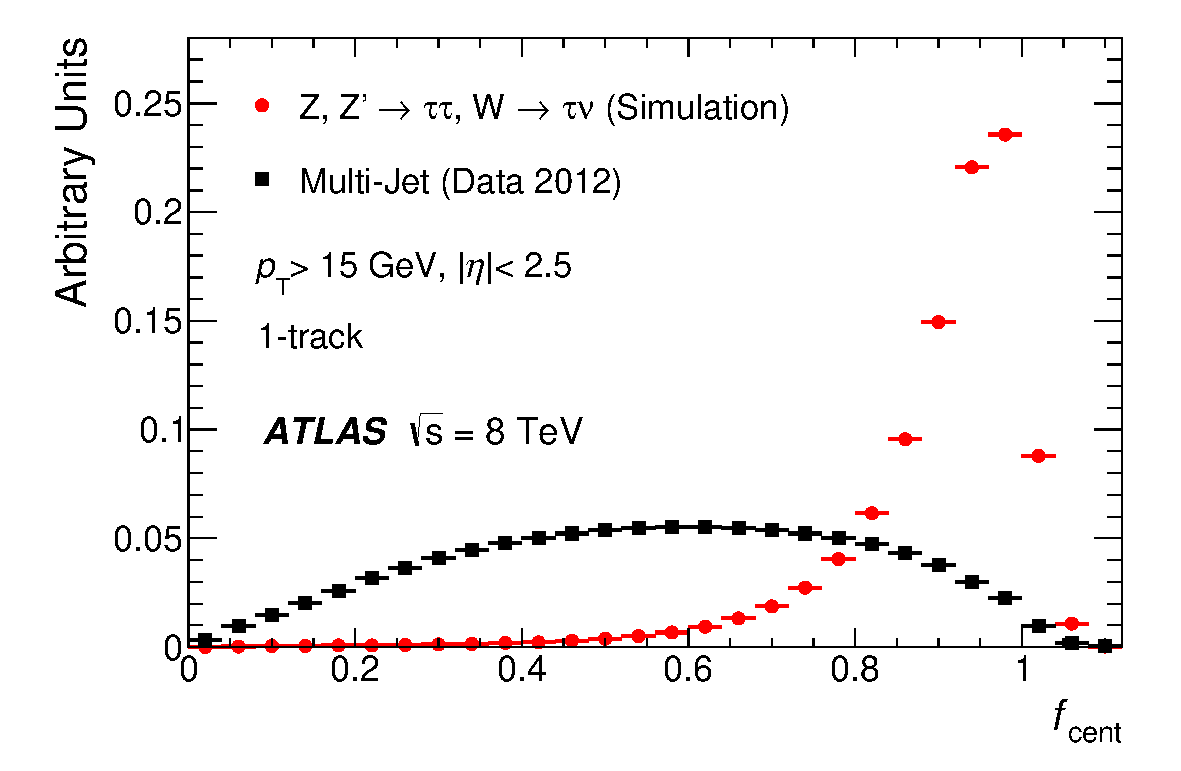
\includegraphics[width=0.48\textwidth]{figures/PERF-2013-06/fig_02a}
  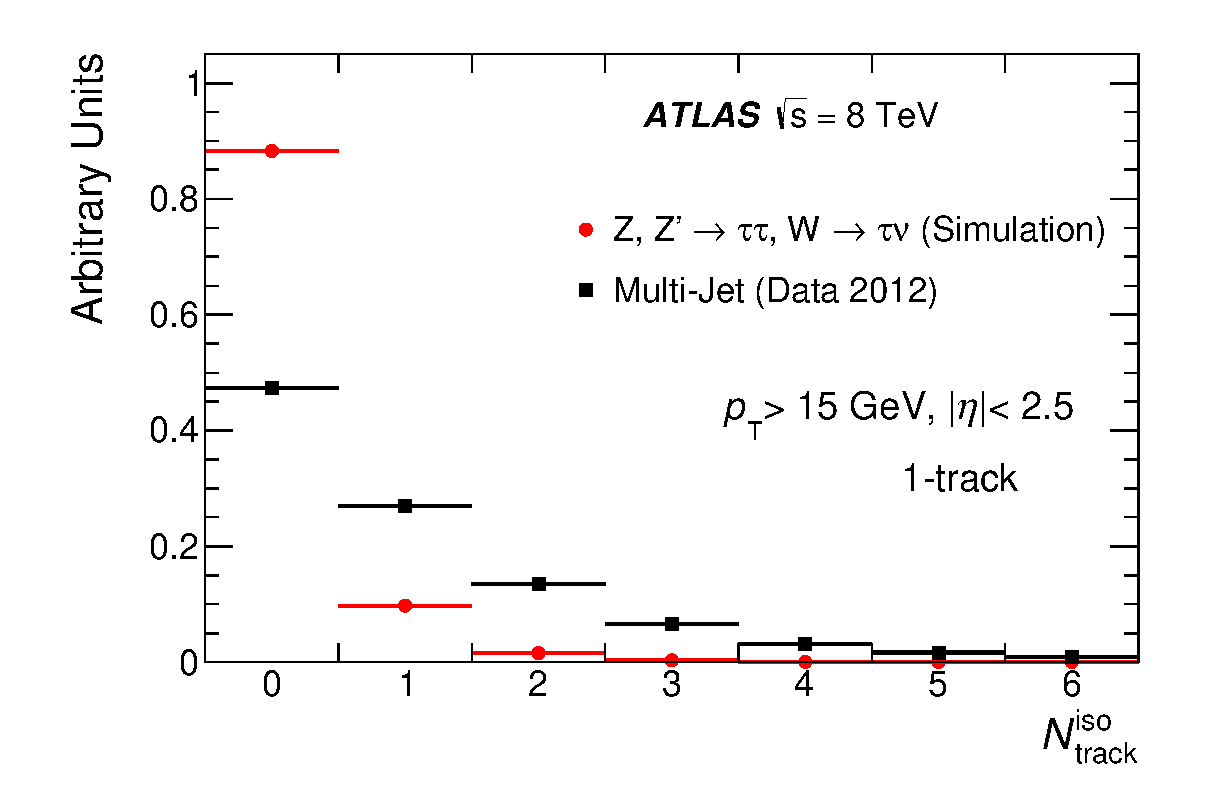
\includegraphics[width=0.48\textwidth]{figures/PERF-2013-06/fig_02b}
  \caption{Signal and background distributions for two of the discriminating variables in the 1-track $\tauh$ jet discrimination algorithm: \centEnergyFrac{} (left) and \numIsoTrack{} (right)~\cite{PERF-2013-06}. The remaining distributions are shown in \cref{apx:tauid}.}
  \label{fig:taus-id1p}
\end{figure}

\begin{figure}[tp]
  \centering
  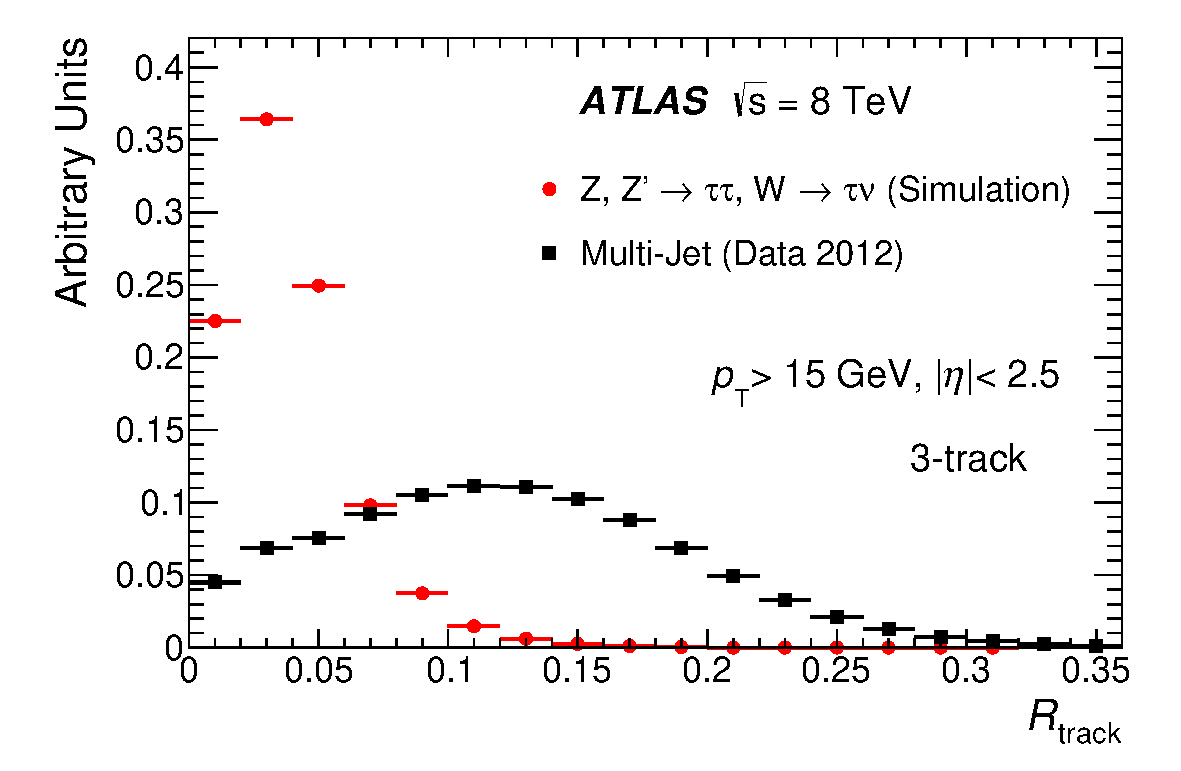
\includegraphics[width=0.48\textwidth]{figures/PERF-2013-06/fig_03a}
  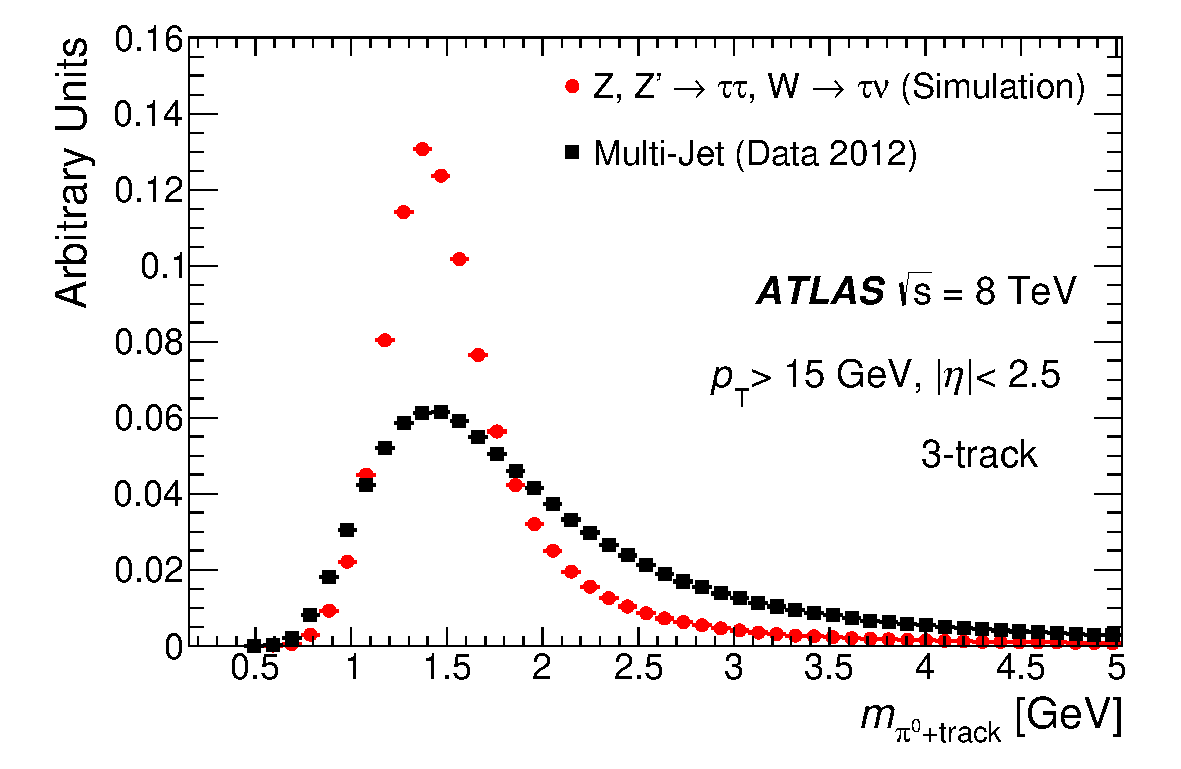
\includegraphics[width=0.48\textwidth]{figures/PERF-2013-06/fig_03b}
  \caption{Signal and background distributions for two of the discriminating variables in the 3-track $\tauh$ jet discrimination algorithm: \trkAvgDist{} (left) and \massTrkPizeroSys{} (right)~\cite{PERF-2013-06}. The remaining distributions are shown in \cref{apx:tauid}.}
  \label{fig:taus-id3p}
\end{figure}

\begin{figure}[tp]
  \centering
  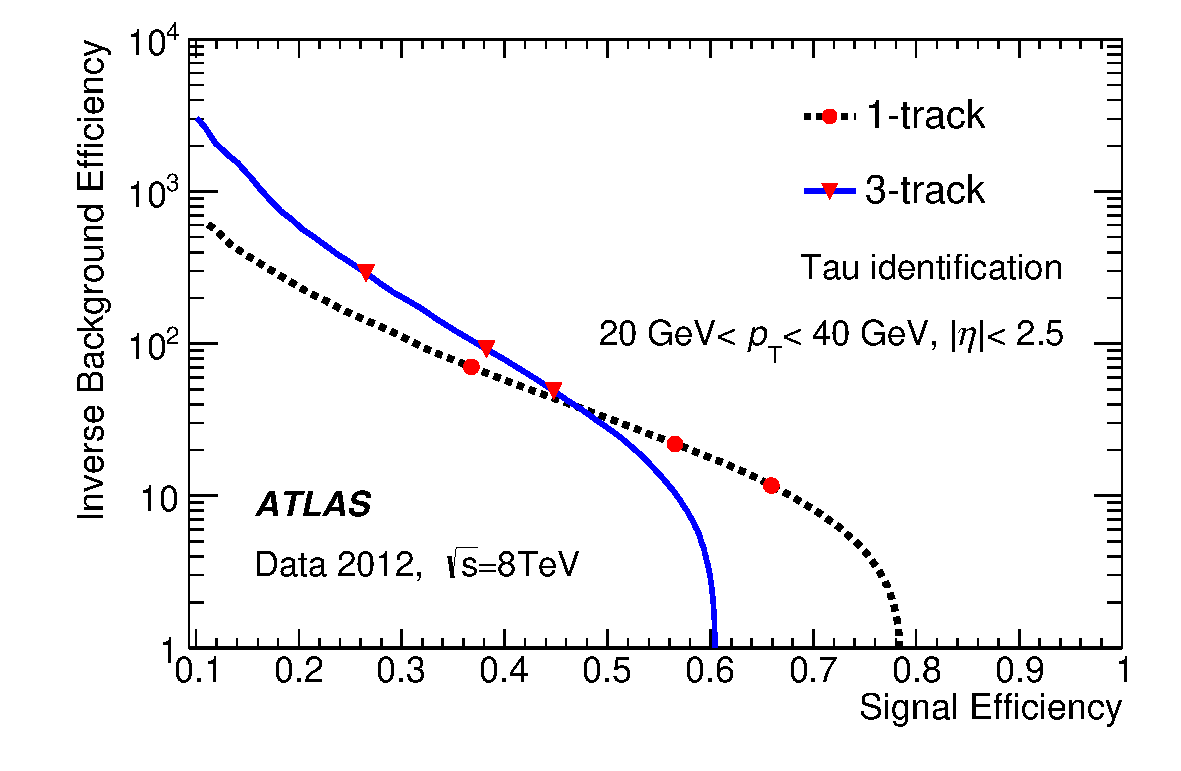
\includegraphics[width=0.48\textwidth]{figures/PERF-2013-06/fig_05a}
  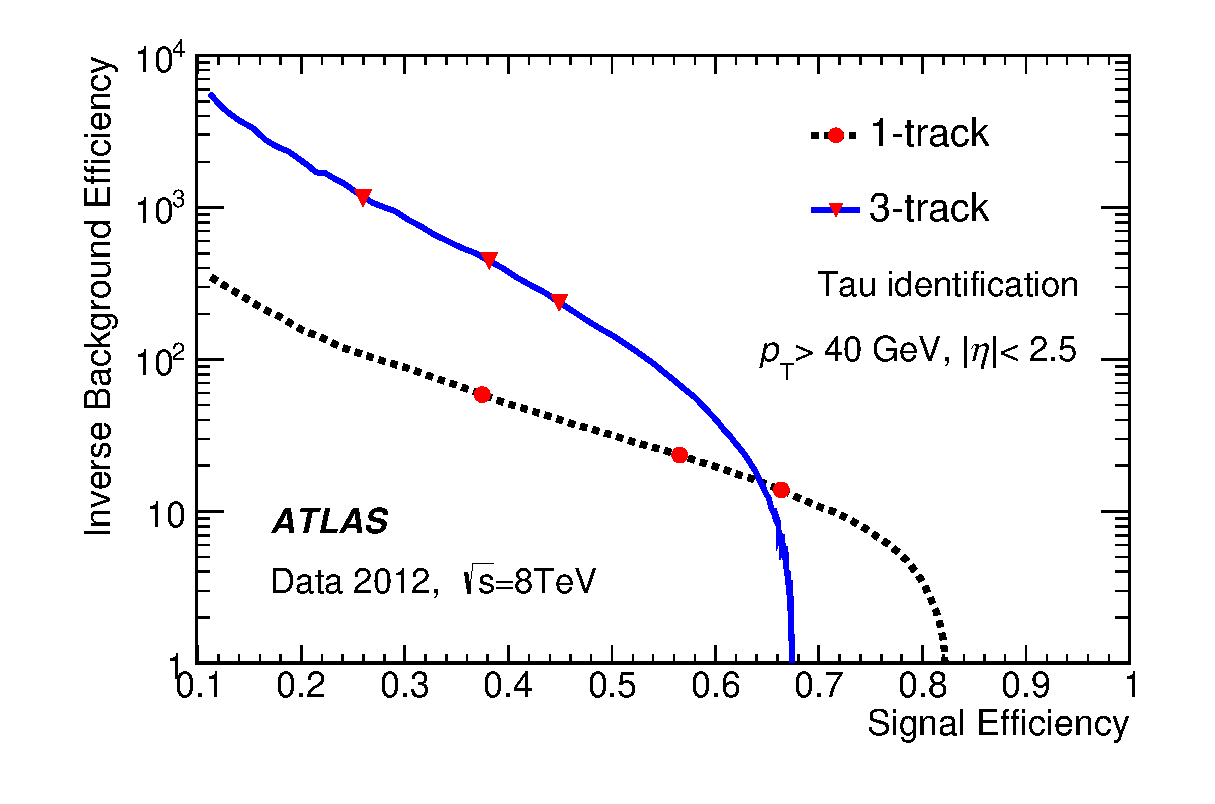
\includegraphics[width=0.48\textwidth]{figures/PERF-2013-06/fig_05b}
  \caption{Signal efficiency versus inverse background efficiency for 1-track and 3-track $\tauh$ jet discrimination algorithms in a lower-$\pt$ regime (left) and higher-$\pt$ regime (right)~\cite{PERF-2013-06}. The loose, medium, and tight operating points are highlighted with red markers.}
  \label{fig:taus-idroc}
\end{figure}

The performance of the jet discrimination algorithms is measured in data and simulation in a $\Ztautaulh$ selection. A tag-and-probe method is used, where the muon from a tau lepton decay is tagged and a $\tauh$ is probed which satisfies topological selections consistent with the $\Ztautaulh$ process. 

To measure the efficiency, templates are built for signal $\tauh$ and background processes of the track multiplicity and fit to data. Correction factors are derived to correct potential mis-modeling in the simulation and shown in \cref{fig:taus-scalefactors}. No significant mis-modeling is observed.

\begin{figure}[tp]
  \centering
  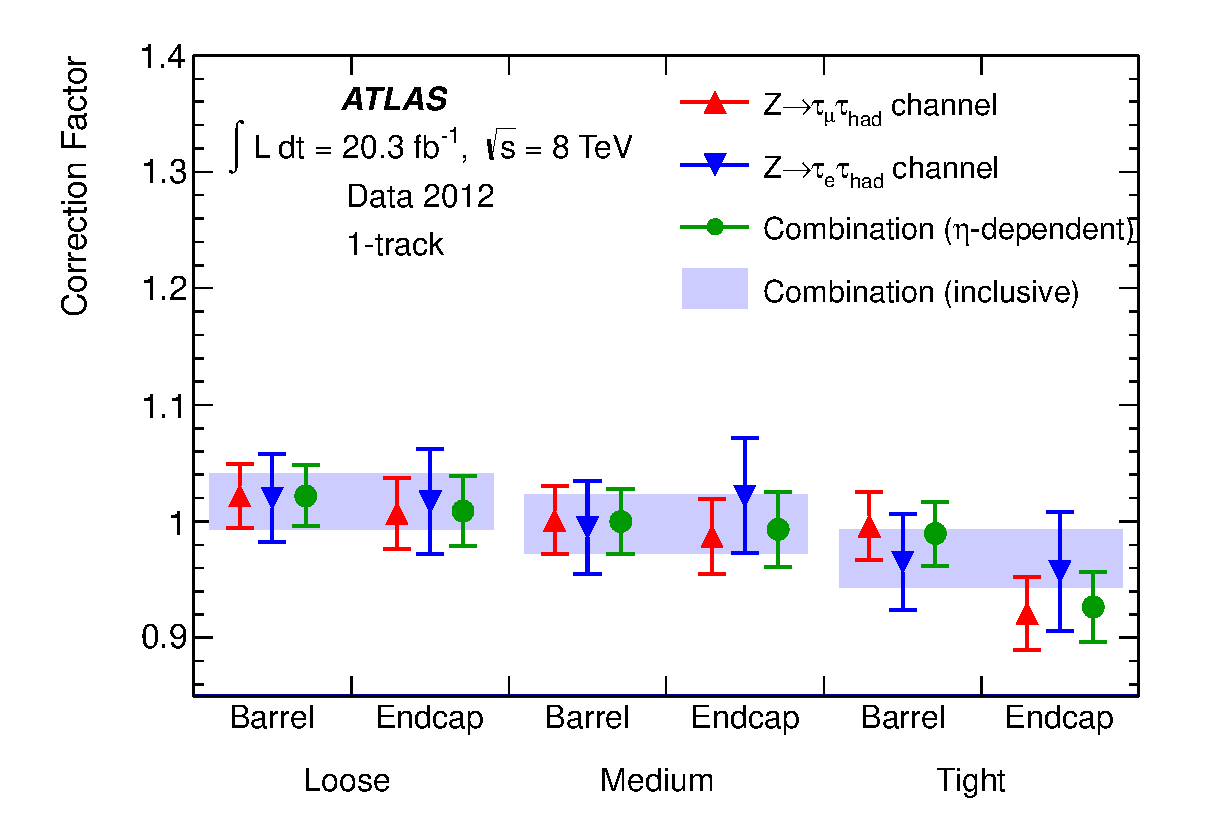
\includegraphics[width=0.48\textwidth]{figures/PERF-2013-06/fig_11a}
  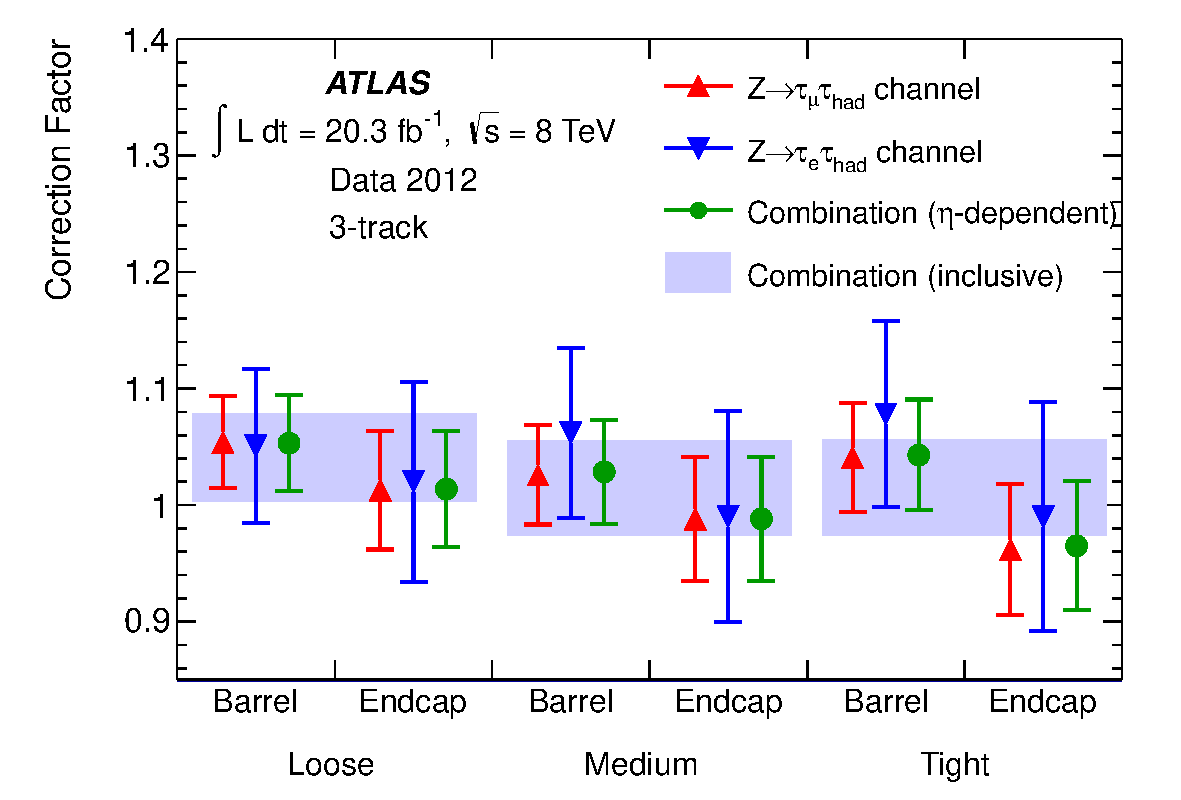
\includegraphics[width=0.48\textwidth]{figures/PERF-2013-06/fig_11b}
  \caption{Correction factors for simulation for the $\tauh$ jet discriminant efficiency for 1-track (left) and 3-track (right) $\tauh$.}
  \label{fig:taus-scalefactors}
\end{figure}

\subsection{Leptons mis-identified as $\tauh$}
\label{sec:taus-leptonfakes}

\subsubsection{Electrons}

The characteristic 1-track signature of $\tauh$ can be mimicked by electrons, even those which fail dedicated electron identification algorithms. This is problematic for $\tautaueh$ analyses because $\Zee$ ($\efake$) peaks in $\mtautau$ near the $\Htautaueh$ mass peak and because high-mass $\ZDYee$ ($\efake$) can have long tails in $\mtautau$.

Despite their similarities, many properties can be used to discriminate electrons from $\tauh$. Electrons tend to produce more transition radiation than $\tauh$, have narrower deposits in the calorimeter, and have shallower deposits in the calorimeter, with rarely any depositions in the hadronic calorimeter. These properties are combined in a multi-variate identification algorithm trained in five regions of $\eta(\tauh)$ to discriminate electrons from simulated $\ZDYee$ against $\tauh$ from simulated $\ZDYtautau$.
%
\begin{description}
    \item[TRT high threshold fraction ($\trtHTFrac$):] \hfill \\
      The ratio of high-threshold to low-threshold hits (including outlier hits) in the TRT for the leading track.
    \item[Pre-sampler and strip fraction ($\pssfraction$):] \hfill \\
      The fraction of cluster energy deposited in the pre-sampler and strips of the EM calorimeter.
    \item[Track-cluster $|\Delta\eta|$:] \hfill \\
      The $|\Delta\eta|$ between the cluster and the leading track.
    \item[Track-cluster $|\Delta\phi|$:] \hfill \\
      The $|\Delta\phi|$ between the cluster and the leading track.
    \item[Hadronic leakage ($\hadLeakEt$):] \hfill \\
      The ratio of energy deposited in the zeroth compartment of the hadronic calorimeter to the lead track momentum.
    \item[EM fraction ($\emFrac$):] \hfill \\
      The fraction of energy deposited in the EM calorimeter.
    \item[Strip maxima ($\Estripmax$):] \hfill \\
      The maximal energy deposited in a $101 \!\times\! 3$ ($\eta, \phi$) window of the strips.
\end{description}
%
\begin{table}[bp] 
  \centering
  \renewcommand{\arraystretch}{1.4}
  \caption{Discriminating variables used in the $\tauh$ electron veto algorithms~\cite{PERF-2013-06,ATLAS-CONF-2013-064,ATLAS-CONF-2012-142}. Some variables are also used in the jet discrimination algorithms.}
  \begin{tabular}{c|ccccc}
                       & \multicolumn{5}{c}{$|\eta(\tauh)|$} \\
  variable             & $0.0 - 0.8$ & $0.8 - 1.37$ & $1.37 - 1.52$ & $1.52 - 2.0$ & $ |\eta| > 2.0$ \\
  \hline
  $\trtHTFrac$         & $\bullet$   & $\bullet$    & $\bullet$     & $\bullet$    &                 \\
  $\pssfraction$       & $\bullet$   & $\bullet$    & $\bullet$     & $\bullet$    & $\bullet$       \\
  $\leadTrackMomFrac$  & $\bullet$   & $\bullet$    & $\bullet$     & $\bullet$    & $\bullet$       \\
  $|\Delta\phi|$       & $\bullet$   & $\bullet$    & $\bullet$     & $\bullet$    & $\bullet$       \\
  $|\Delta\eta|$       & $\bullet$   & $\bullet$    & $\bullet$     & $\bullet$    & $\bullet$       \\
  $\hadLeakEt$         & $\bullet$   & $\bullet$    & $\bullet$     & $\bullet$    & $\bullet$       \\
  $\emFrac$            & $\bullet$   & $\bullet$    & $\bullet$     & $\bullet$    & $\bullet$       \\
  $\Estripmax/\pt$     & $\bullet$   & $\bullet$    &               &              &                 \\
  $\isoFrac$           &             & $\bullet$    &               & $\bullet$    & $\bullet$       \\
  $\centEnergyFrac$    & $\bullet$   &              & $\bullet$     &              &                 \\
\end{tabular}


  \label{tab:taus-evetovars}
\end{table}

\begin{figure}[tp]
  \centering
  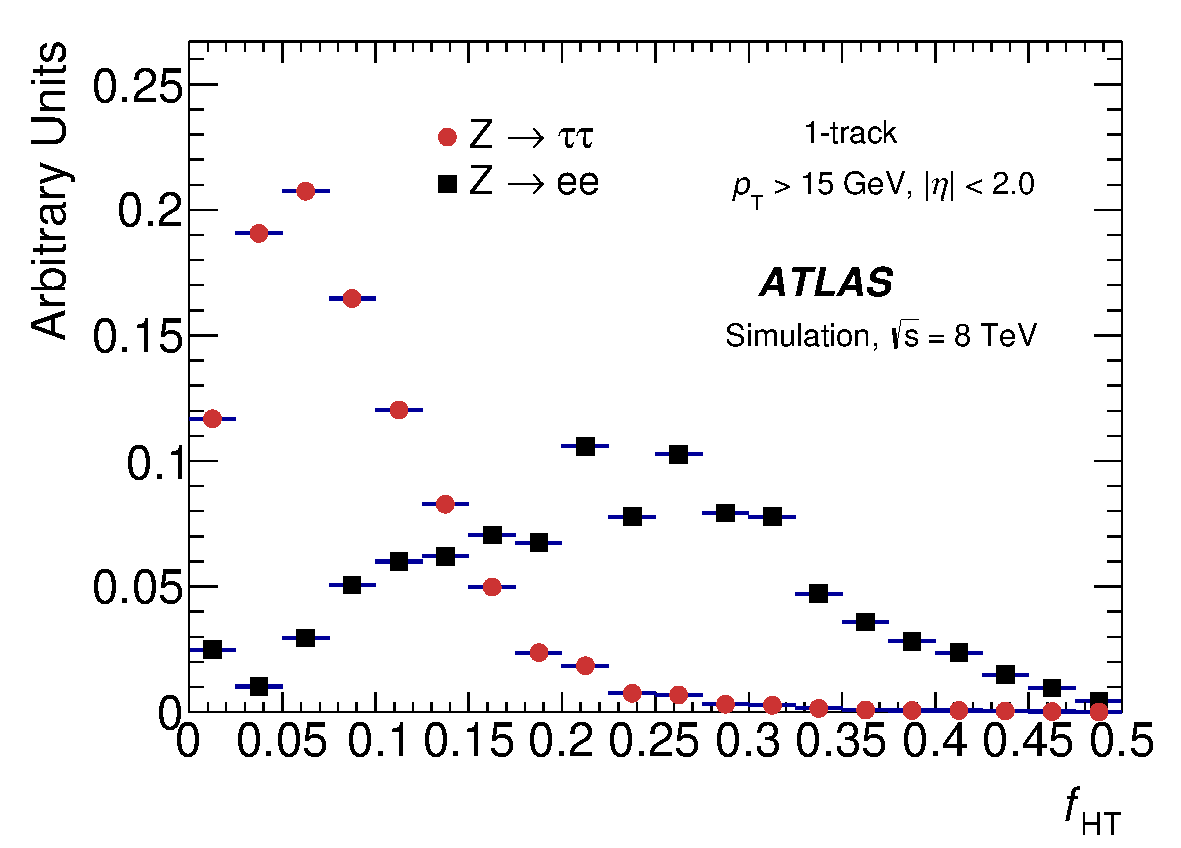
\includegraphics[width=0.48\textwidth]{figures/PERF-2013-06/fig_08a}
  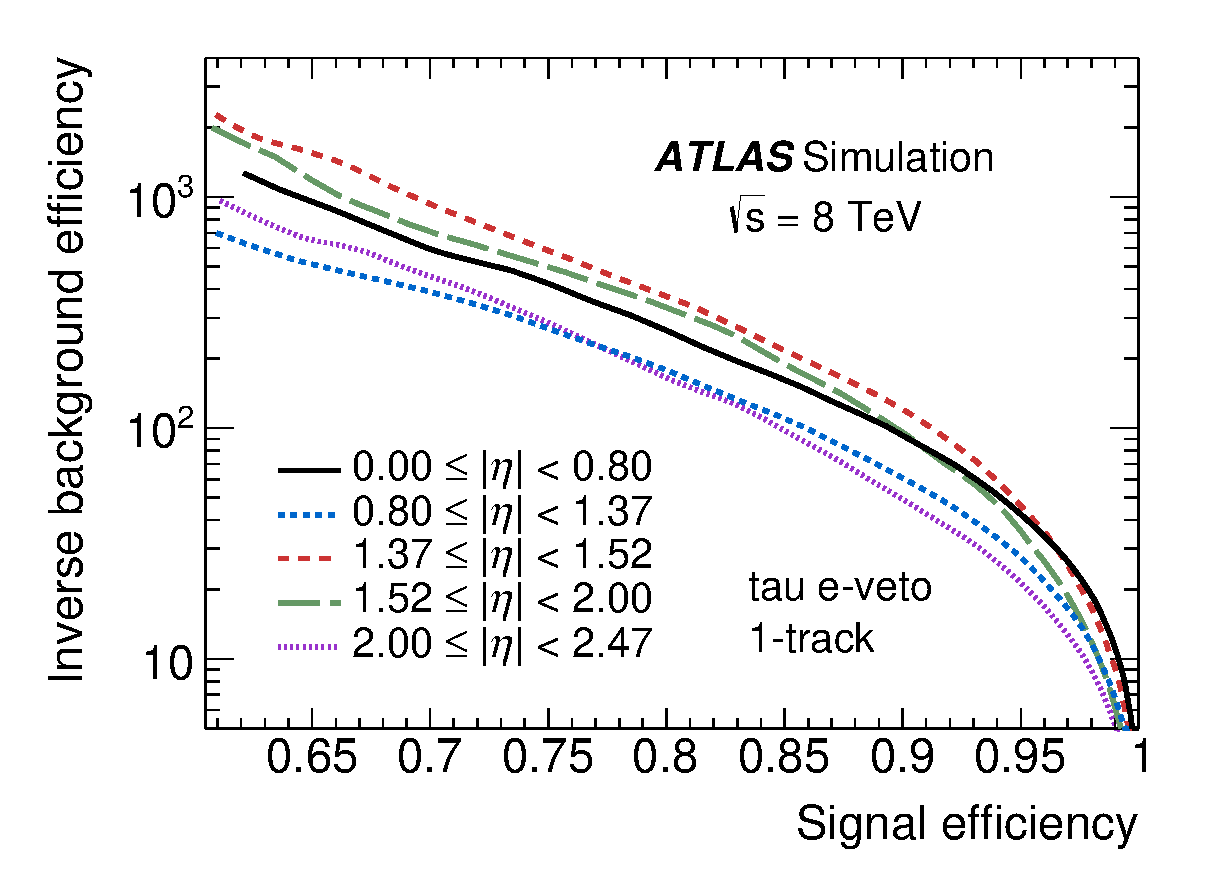
\includegraphics[width=0.48\textwidth]{figures/PERF-2013-06/fig_09}
  \caption{Signal and background distribution for one of the variables in the $\tauh$ electron discrimination algorithm: the TRT high threshold fraction (left), and signal efficiency versus inverse background efficiency for the algorithm (right)~\cite{PERF-2013-06}.}
  \label{fig:taus-electronfakes1}
\end{figure}

The performance of the electron discriminators is evaluated in data and simulation using a $\Zee$ tag-and-probe technique, where one identified electron is tagged and a $\tauh$ candidate is probed where the mass of the electron-$\tauh$ pair is consistent with the $Z$ mass. This measurement can be challenging because few $\efake$ survive the electron discrimination algorithms. The characteristic peak in $\mvis$ is shown in \cref{fig:taus-electronfakes2} before and after application of the algorithms.

In the 2012 version of the electron discriminator, a mis-modeling in simulation is found in the forward region regarding the energy deposited in the third layer of the EM calorimeter, which propagates to the discriminator via $\emFrac$. The mis-modeling is ameliorated in the 2013 version by redefining $\emFrac$ to depend less strongly on the third layer deposition, and the modeling is improved, as shown in \cref{fig:taus-electronfakes3}.

\begin{figure}[tp]
  \centering
  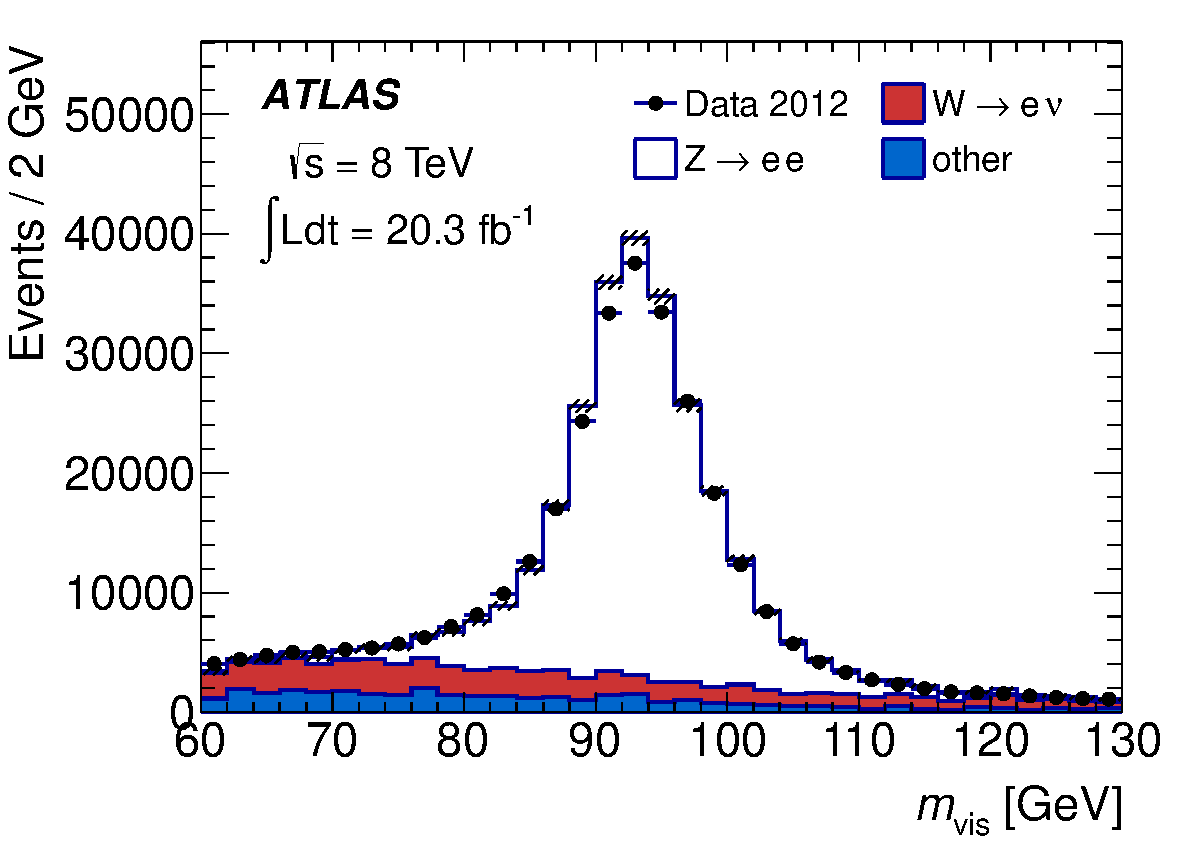
\includegraphics[width=0.48\textwidth]{figures/PERF-2013-06/fig_14a}
  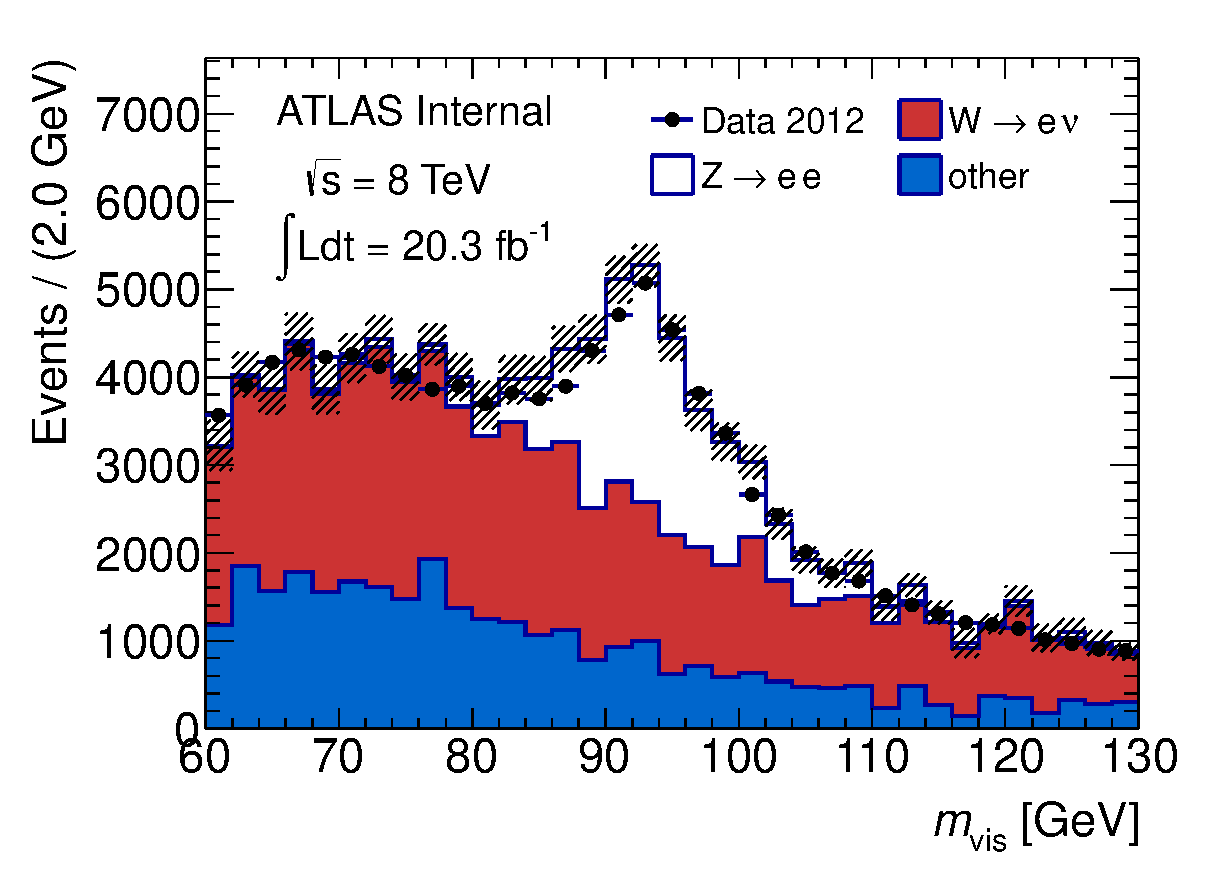
\includegraphics[width=0.48\textwidth]{figures/PERF-2013-06/eveto_mvis_mediumID_loosePPOLR_looseeveto}
  \caption{The visible mass $m_{e\tauh}$ in a $\Zee$ selection in data after requiring the $\tauh$ candidate pass the medium jet discrimination algorithm and not overlap spatially with a tight identified electron (left)~\cite{PERF-2013-06} and after additionally requiring the $\tauh$ pass the loose $\tauh$ electron discrimination algorithm (right).}
  \label{fig:taus-electronfakes2}
\end{figure}

\begin{figure}[tp]
  \centering
  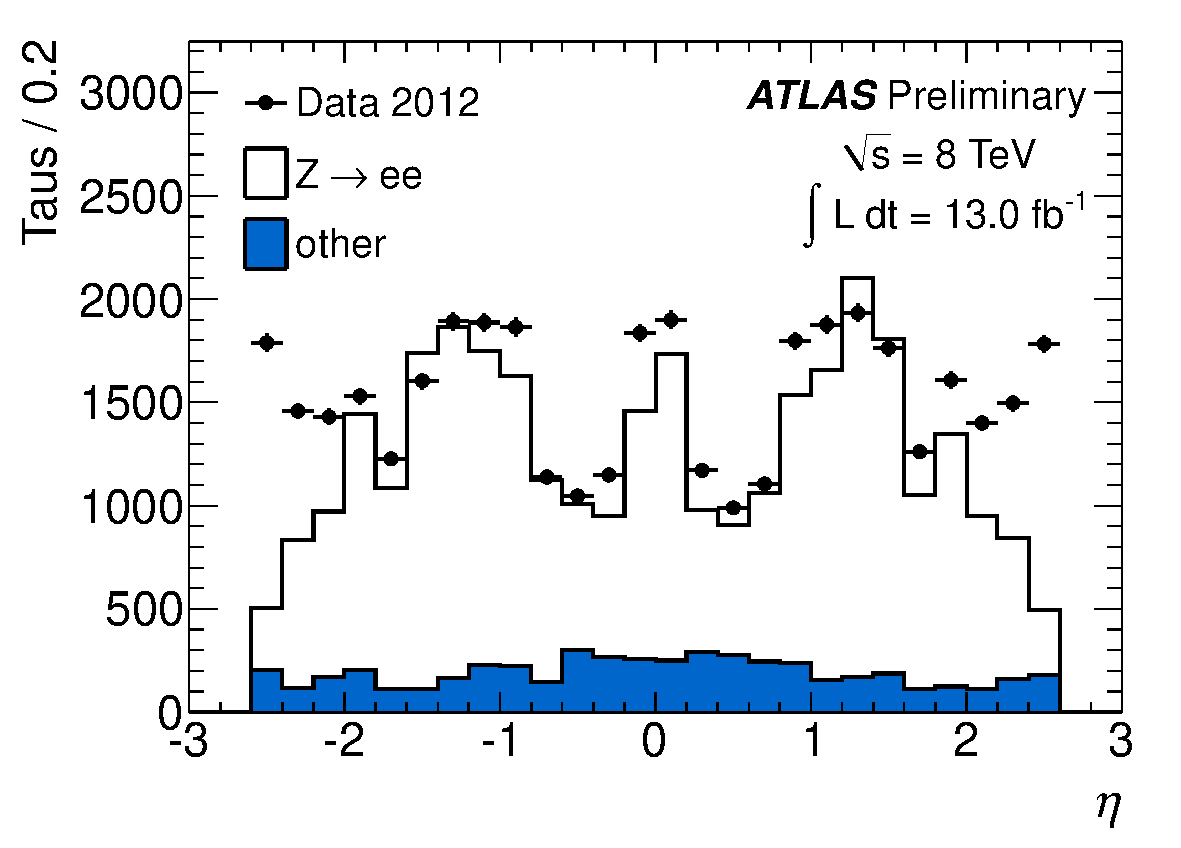
\includegraphics[width=0.48\textwidth]{figures/ATLAS-CONF-2013-064/fig_22b}
  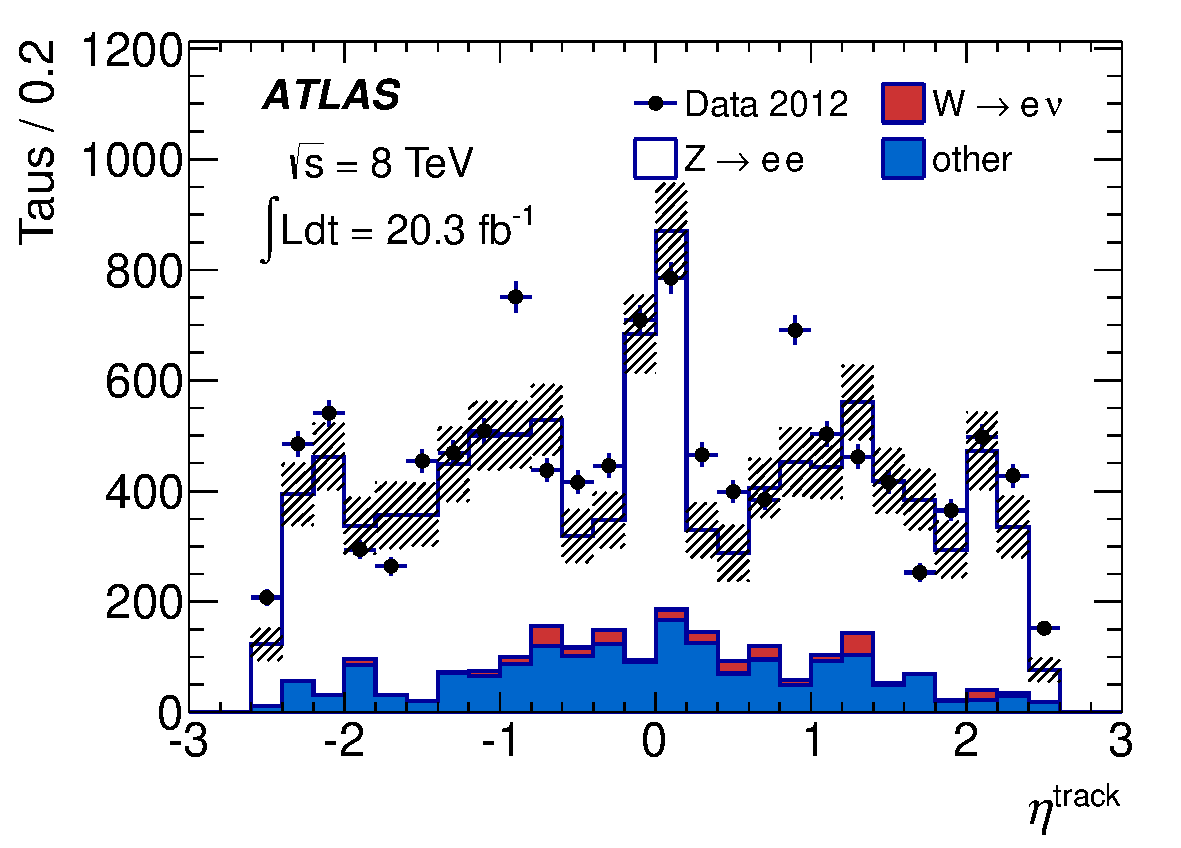
\includegraphics[width=0.48\textwidth]{figures/PERF-2013-06/fig_14b}
  \caption{The pseudorapidity $\eta(\tauh)$ in a $\Zee$ selection in data after requiring the $\tauh$ candidate pass the medium jet discrimination algorithm, not overlap spatially with a tight identified electron, and pass the loose $\tauh$ electron discrimination algorithm from 2012 (left)~\cite{ATLAS-CONF-2013-064} and 2013 (right)~\cite{PERF-2013-06}. Statistical uncertainty is not shown on the left. The modeling is improved in the forward region.}
  \label{fig:taus-electronfakes3}
\end{figure}

\subsubsection{Muons}

The characteristic 1-track signature of $\tauh$ can also be mimicked by muons. This is more rare than $\efake$ mis-identification since muons are minimum ionizing particles and do not often deposit sufficient energy in the calorimeters to seed a $\tauh$ candidate. But $\Zmumu$ ($\mfake$) can nonetheless be a problem for $\tautaumh$ final states for the same reasons as $\Zee$ is problematic for $\tautaueh$ final states.

Studies of $\Zmumu$ simulation indicate most (60\%) $\mfake$ have a cluster in the calorimeter from photon FSR. The remaining are assumed to undergo sufficient ionization in the hadronic calorimeter to create a cluster. Only 2\% of $\mfake$ are not reconstructed as a muon candidate. Most of these $\mfake$ occur in a region of $\eta$ which is poorly covered by the muon system, and some occur because they are too low $\pt$ for the muon reconstruction algorithms.
%
\begin{table}[bp] 
  \centering
  \renewcommand{\arraystretch}{1.4}
  \caption{A breakdown of how $\mfake$ occur, both in the case of all $\mfake$ and only those which fail the muon reconstruction.}
  \begin{tabular}{c|cc|cc}
                             & \multicolumn{2}{c}{cluster from:}     &                     &                      \\
  type of $\mfake$           & FSR $\gamma$ & detector (e.g., brem.) & true $\pt < $ 5 GeV & true $|\eta| < $ 0.1 \\
  \hline
  all                        & 59\%         & 41\%                   & 2\%                 & 4\%                  \\
  not reconstructed as $\mu$ & 60\%         & 40\%                   & 20\%                & 60\%                 \\
\end{tabular}


  \label{tab:taus-muonfakes}
\end{table}
%
These properties are shown in \cref{fig:taus-muonfakes-1} and \cref{fig:taus-muonfakes-2}.

\begin{figure}[tp]
  \centering
  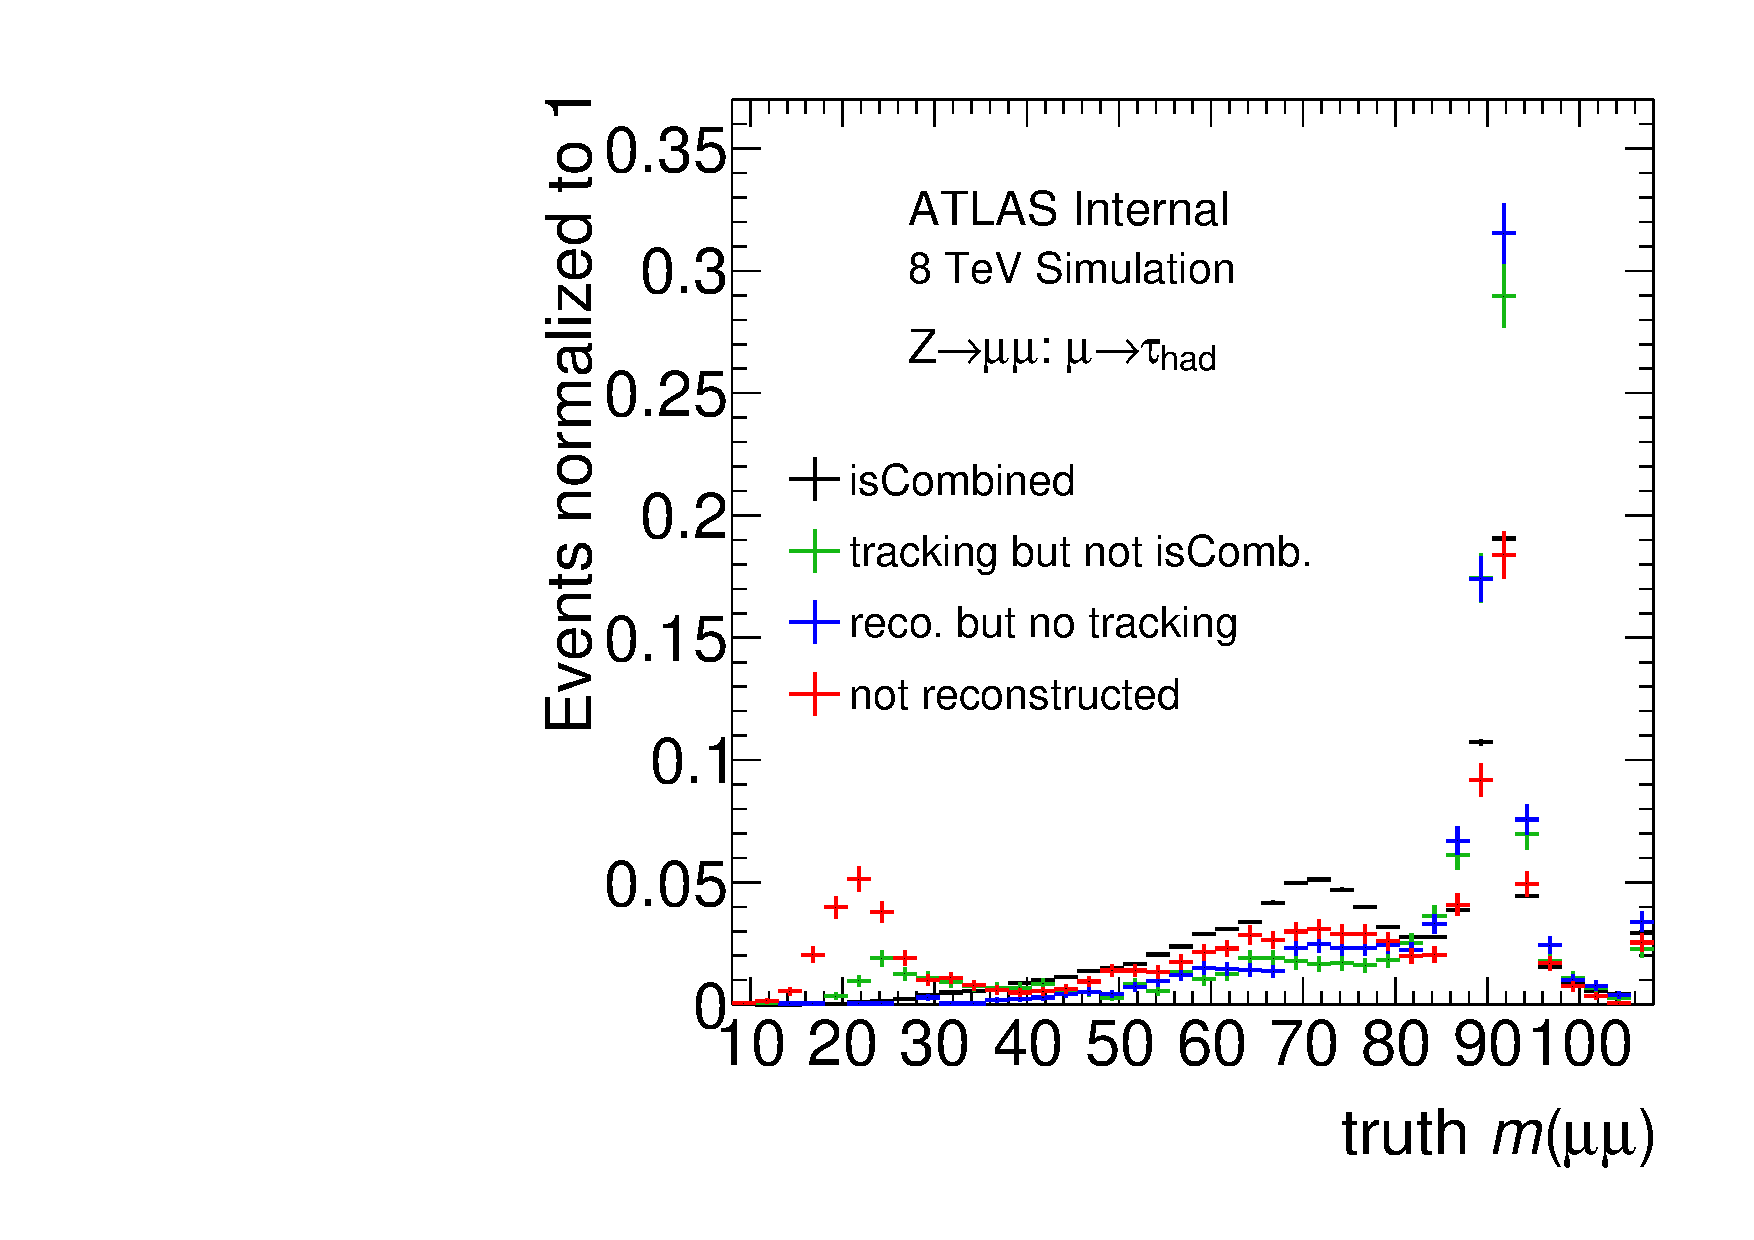
\includegraphics[width=0.48\textwidth]{figures/tauperformance/muonfakes_mll}
  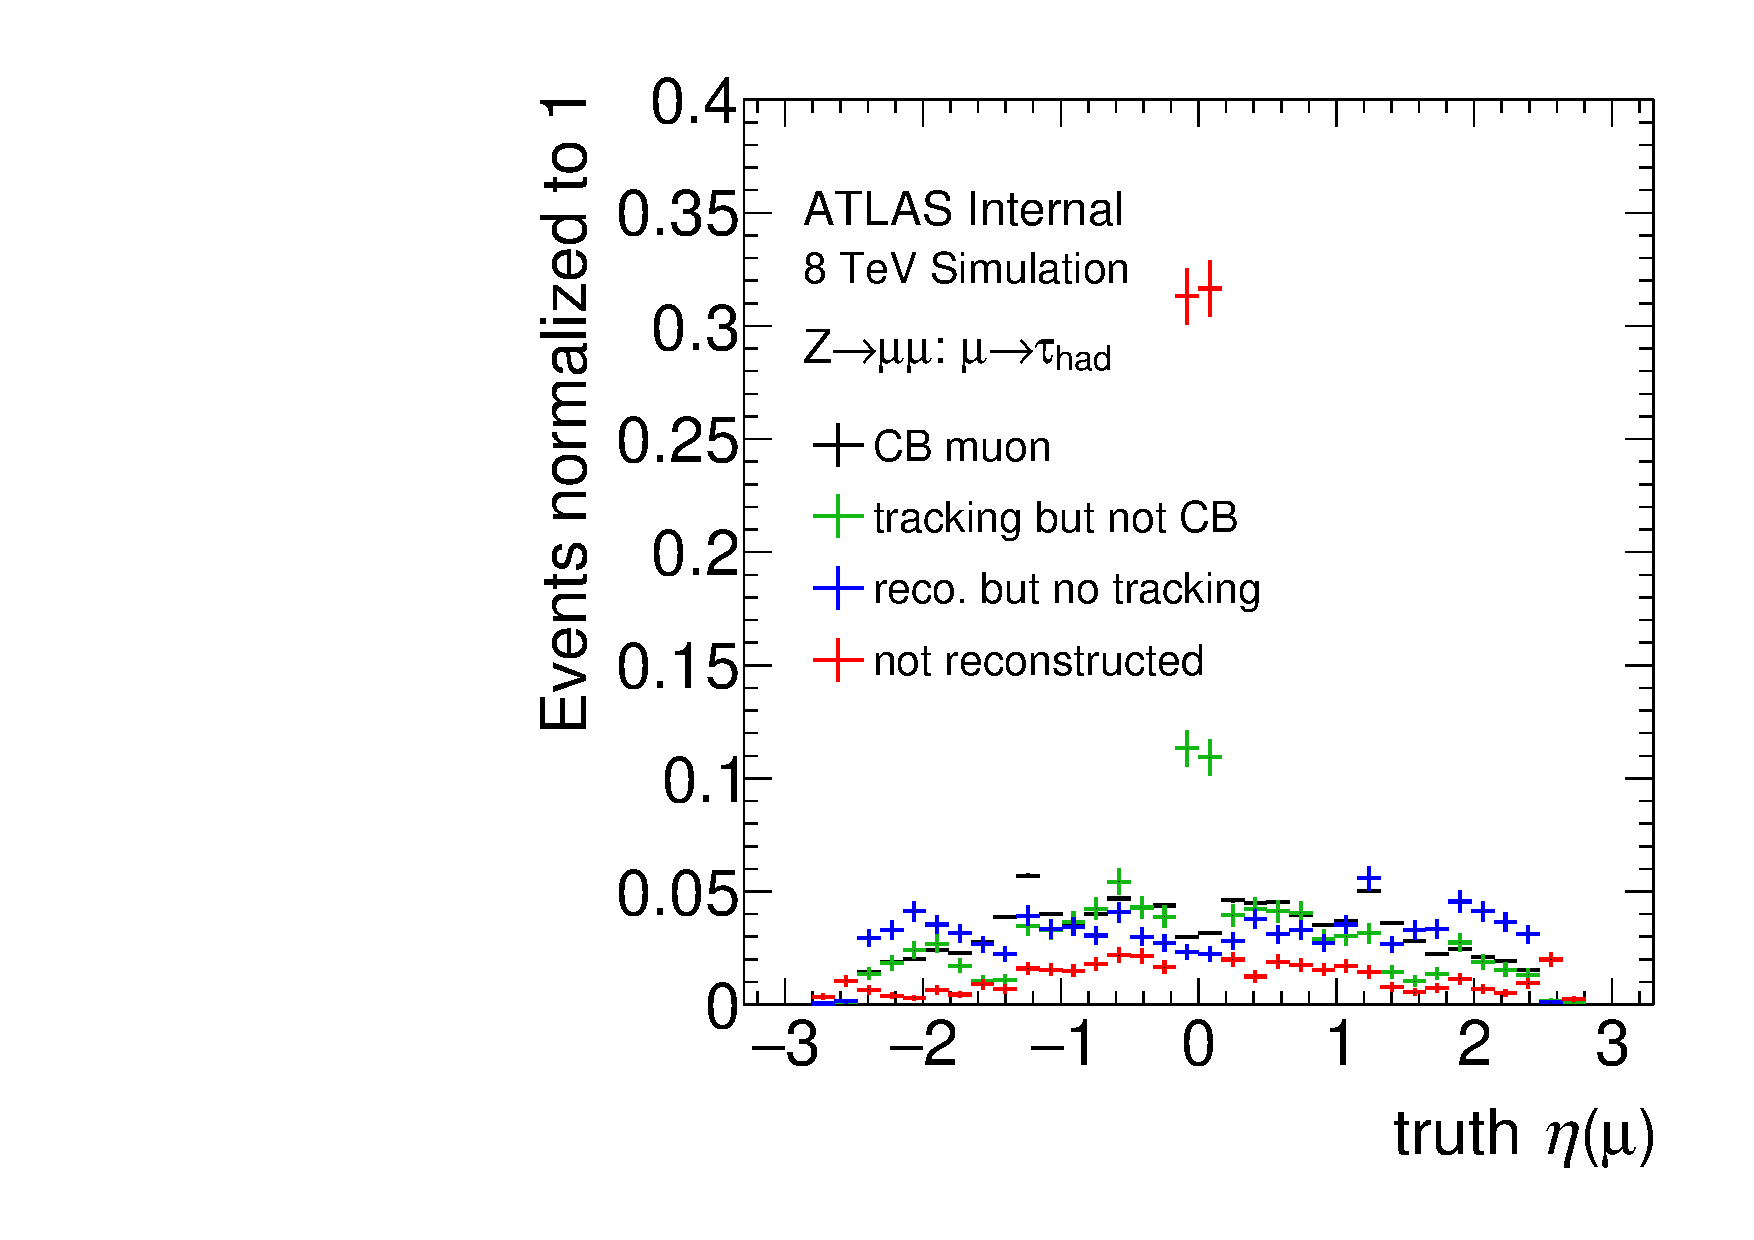
\includegraphics[width=0.48\textwidth]{figures/tauperformance/muonfakes_eta}
  \caption{True $m_{\mu\mu}$ (left) and $\eta(\mu)$ (right) in $\Zmm$ events where a muon is mis-identified as a $\tauh$. The muons are split into \texttt{combined} muons (black), muons which pass tracking requirements but fail \texttt{combined} requirements (green), are reconstructed but fail tracking requirements (blue), and are not reconstructed (red). A large fraction of non-reconstructed muons have $|\eta| \approx 0$, which is a poorly covered region of the muon system.}
  \label{fig:taus-muonfakes-1}
\end{figure}

\begin{figure}[tp]
  \centering
  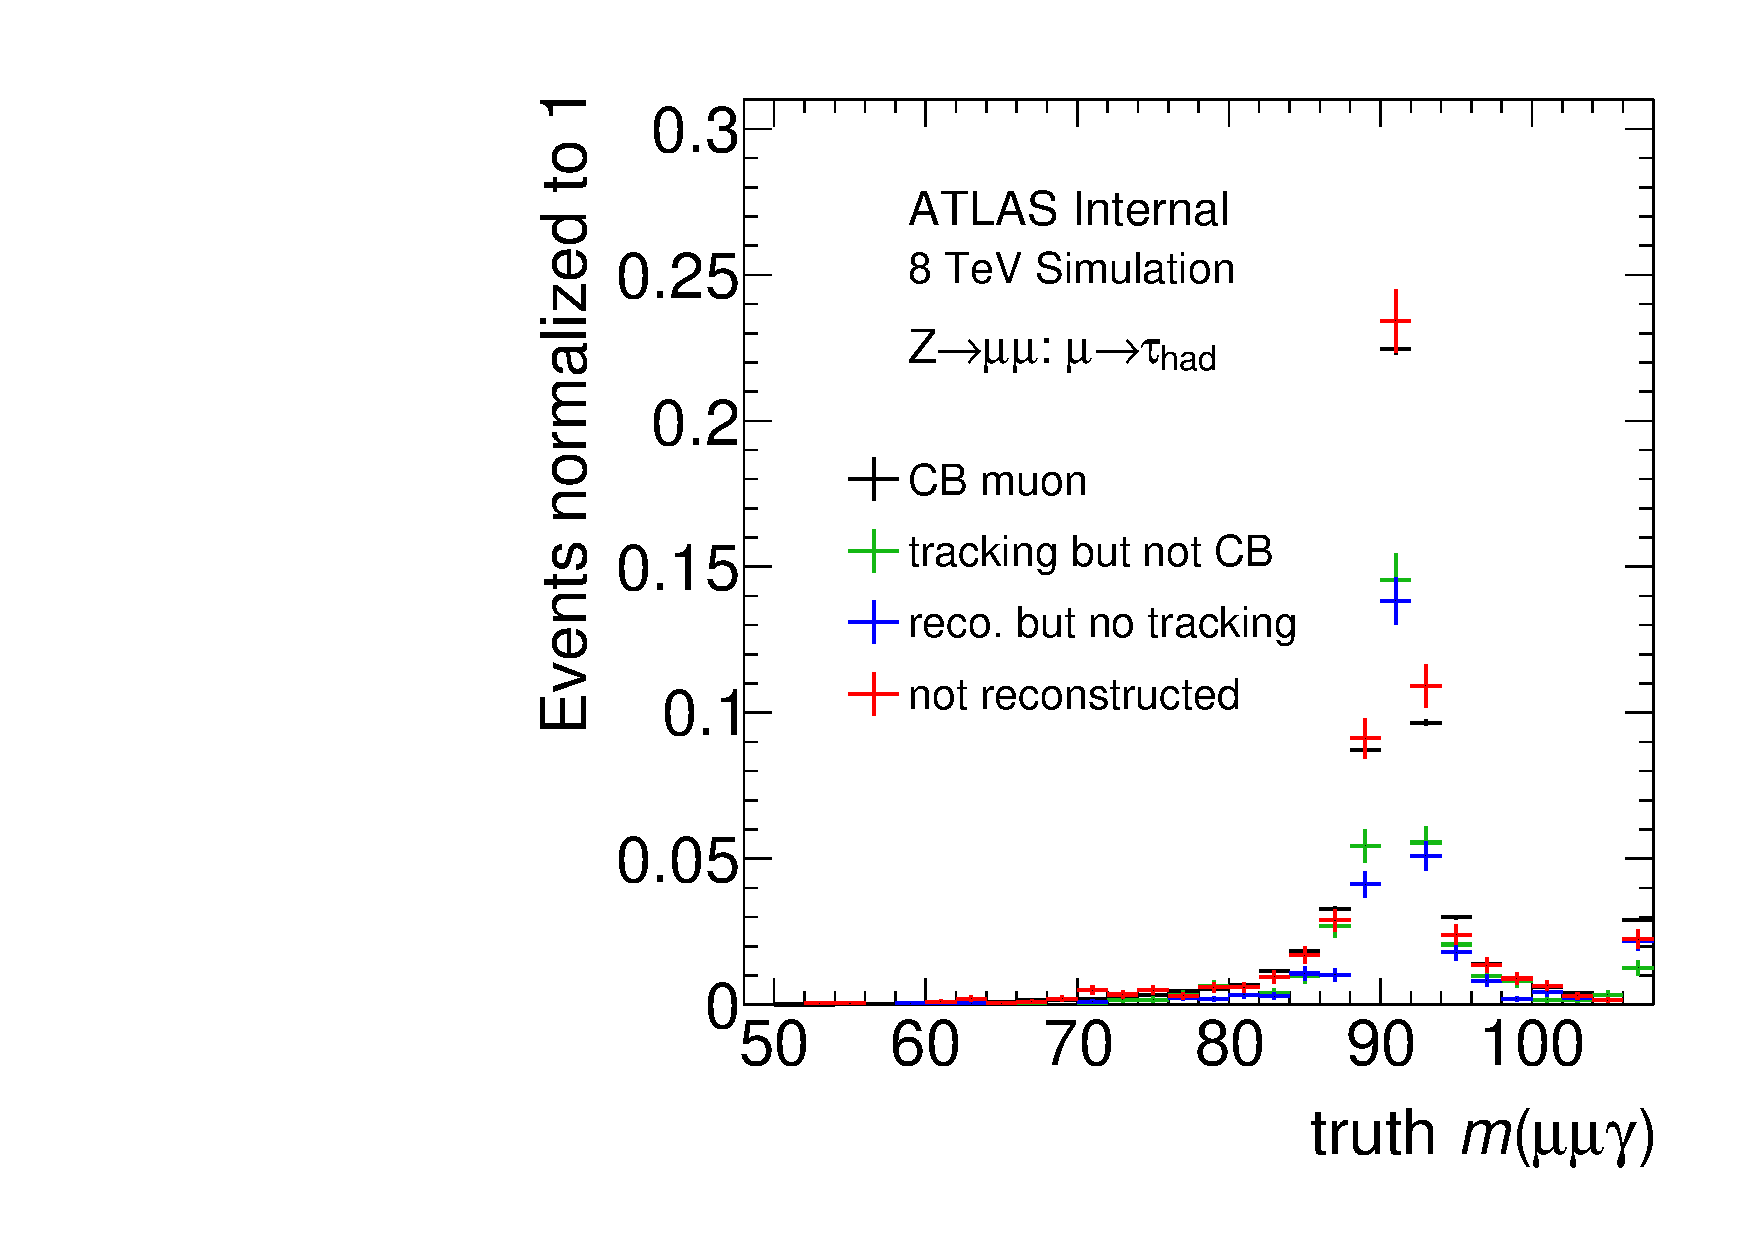
\includegraphics[width=0.48\textwidth]{figures/tauperformance/muonfakes_mlly}
  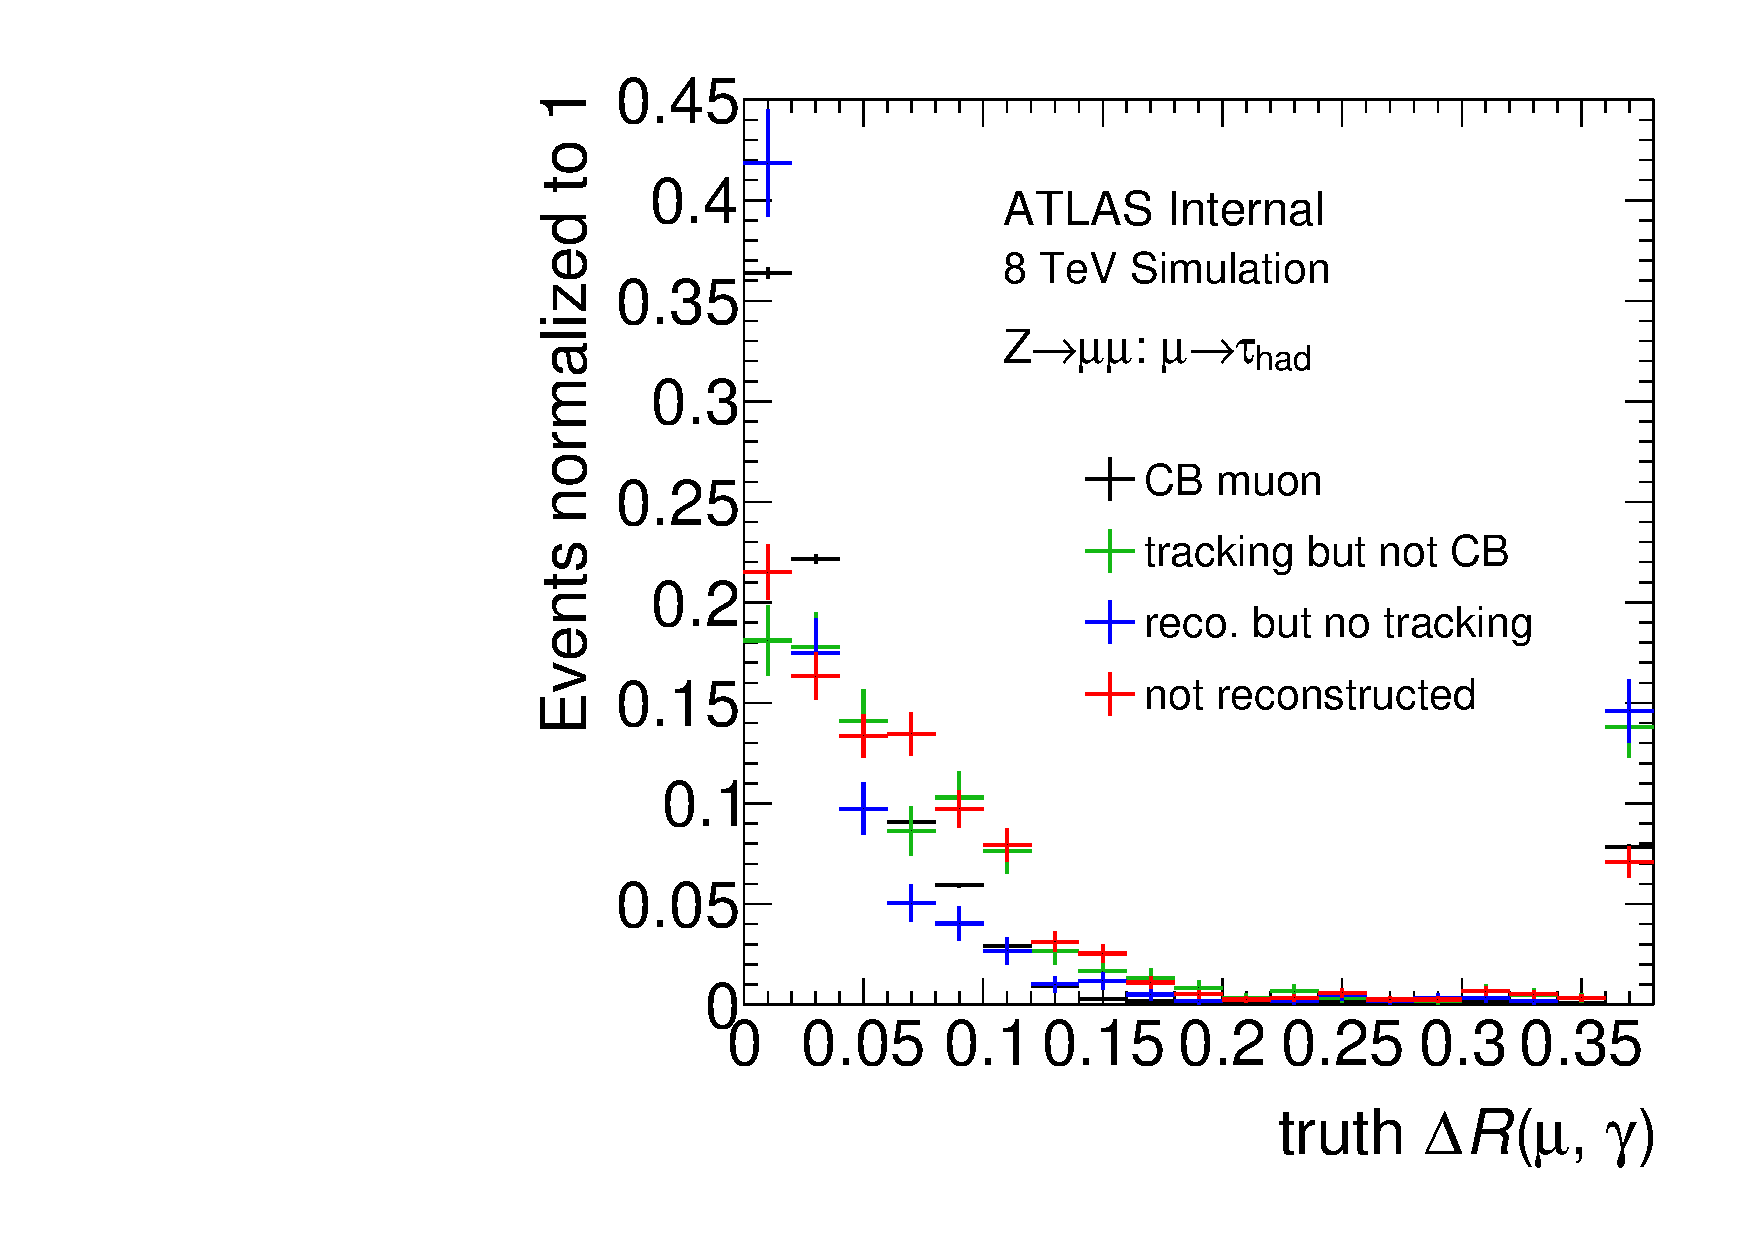
\includegraphics[width=0.48\textwidth]{figures/tauperformance/muonfakes_dR}
  \caption{True $m_{\mu\mu\gamma}$ (left) and $\Delta R(\mu,\ \gamma)$ (right) in $\Zmm$ events where a muon is mis-identified as a $\tauh$ and a true FSR photon is associated to the muon. The muons are split into \texttt{combined} muons (black), muons which pass tracking requirements but fail \texttt{combined} requirements (green), are reconstructed but fail tracking requirements (blue), and are not reconstructed (red).}
  \label{fig:taus-muonfakes-2}
\end{figure}

In physics analysis, $\mfake$ are typically rejected by requiring a $\tauh$ candidate not overlap with an identified muon and that it pass an additional, dedicated muon veto. These rejection criteria are re-optimized in 2014 for better $\mfake$ suppression and simultaneously better true $\tauh$ efficiency. The updated rejection removes the dedicated muon veto, which costs $\approx\!5\%$ efficiency for true $\tauh$, and tightens the overlap criteria such that $\tauh$ candidates are rejected if they overlap with any reconstructed muon above 2 GeV. The improved rejection of this criteria is shown in \cref{fig:taus-muonfakes3}.

\begin{figure}[tp]
  \centering
  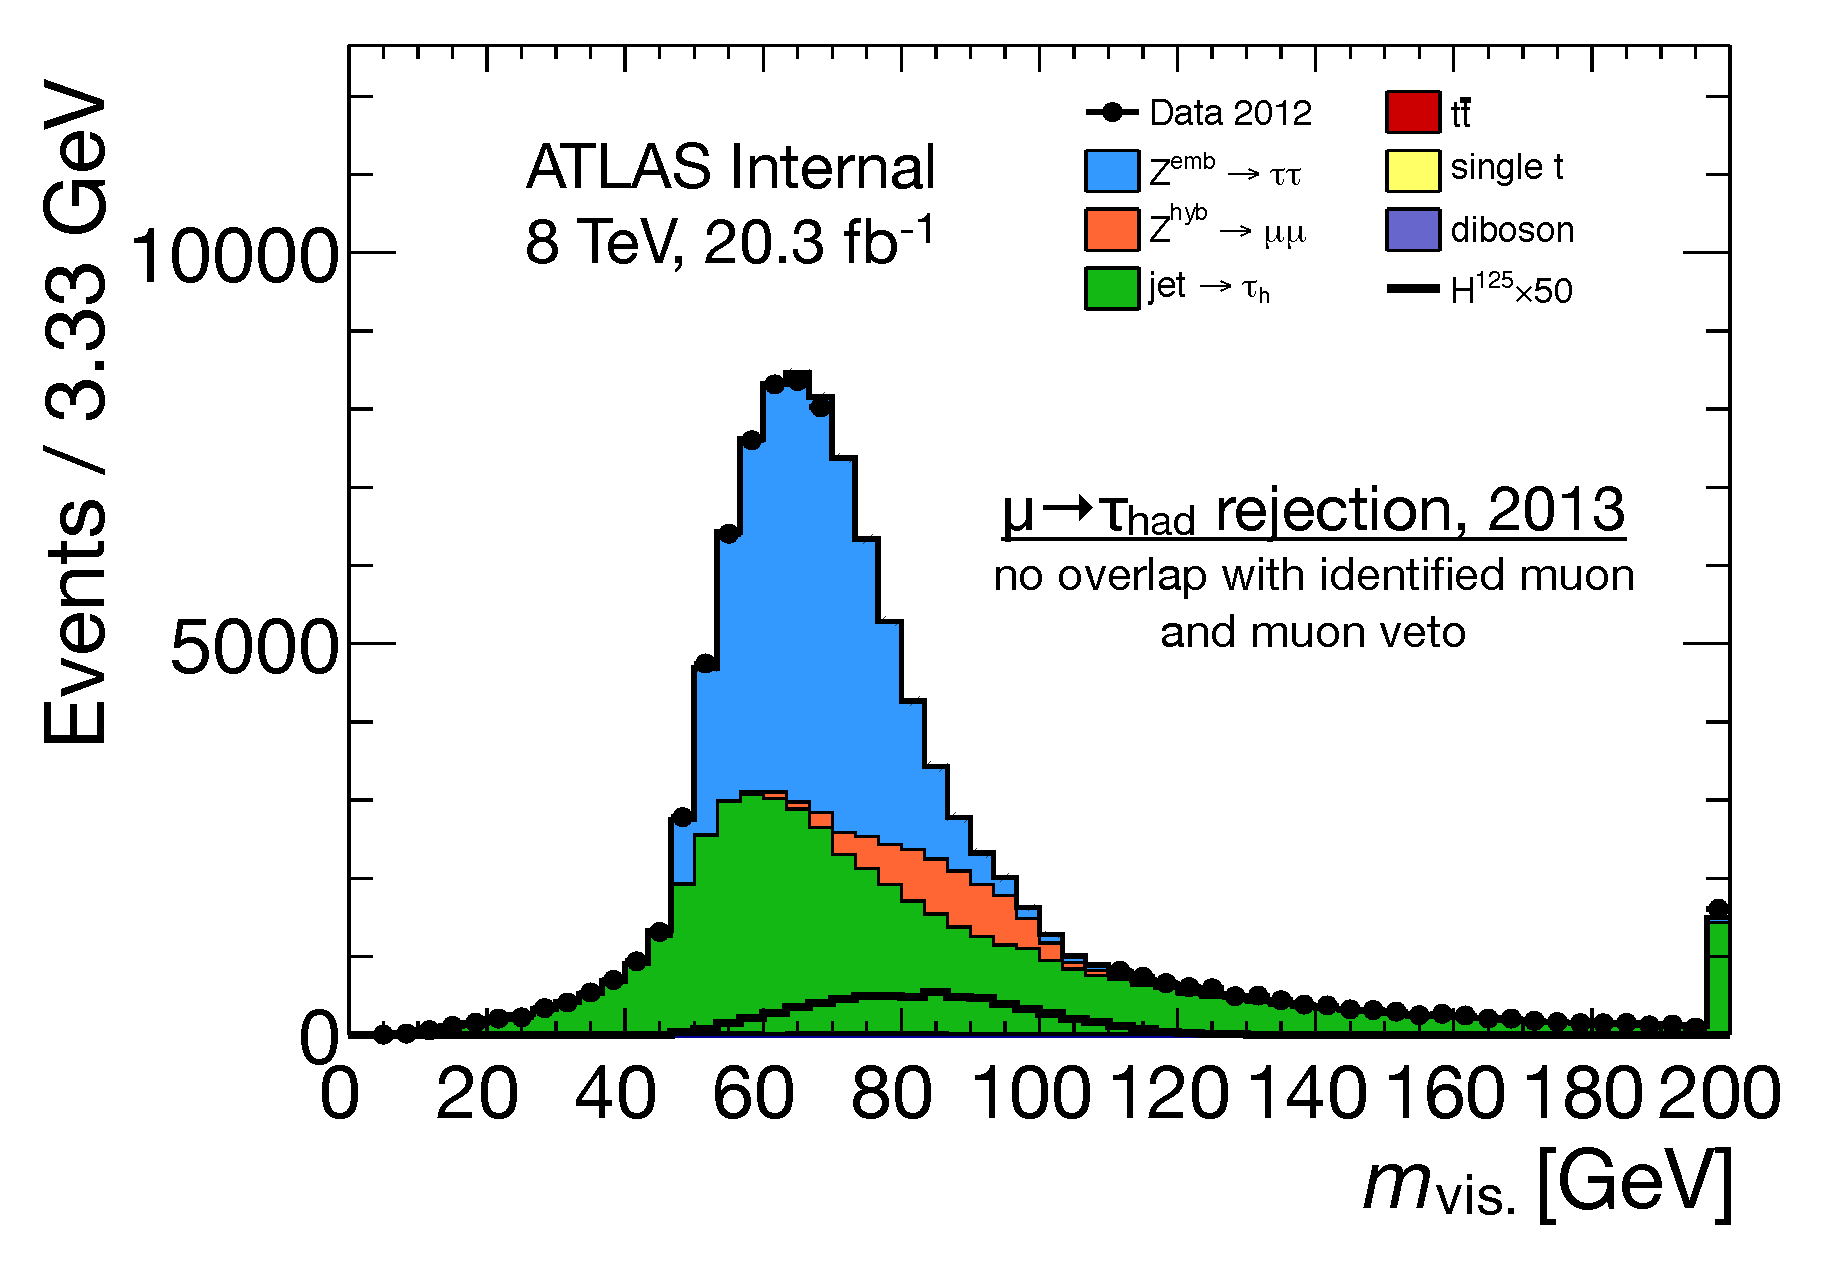
\includegraphics[width=0.48\textwidth]{figures/tauperformance/muonrejection_2013}
  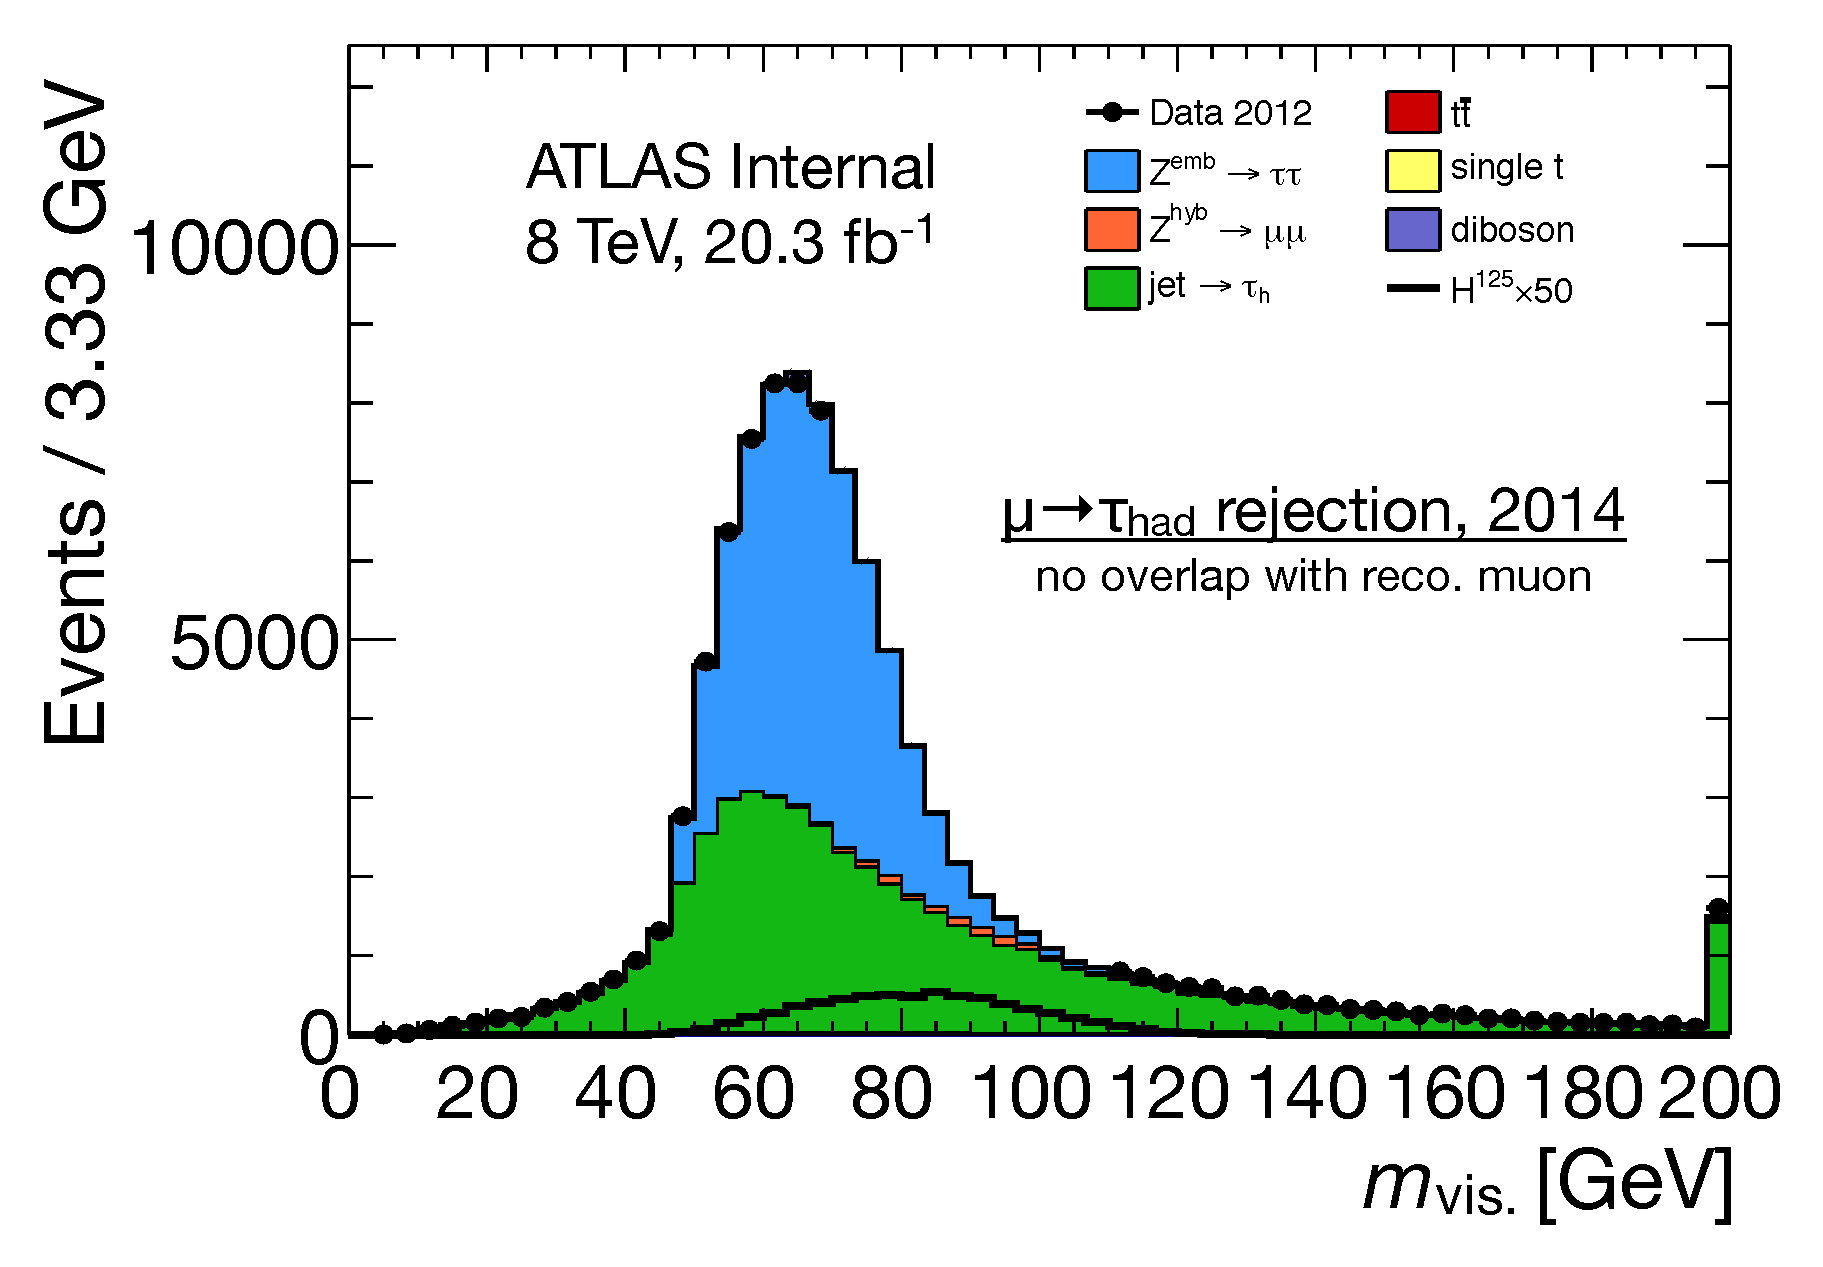
\includegraphics[width=0.48\textwidth]{figures/tauperformance/muonrejection_2014}
  \caption{Data and prediction in a $\Ztautaumh$ selection, where $\Zmumu$ ($\mfake$) is shown in orange, for 2013 (left) and 2014 (right) versions of $\mfake$ rejection techniques. Overlapping muon candidates in the 2013 version are required to fulfill tracking goodness as a form of identification. The $\Zmumu$ ($\mfake$) is reduced significantly in the 2014 version.}
  \label{fig:taus-muonfakes3}
\end{figure}



